\documentclass[twoside]{book}

% Packages required by doxygen
\usepackage{fixltx2e}
\usepackage{calc}
\usepackage{doxygen}
\usepackage[export]{adjustbox} % also loads graphicx
\usepackage{graphicx}
\usepackage[utf8]{inputenc}
\usepackage{makeidx}
\usepackage{multicol}
\usepackage{multirow}
\PassOptionsToPackage{warn}{textcomp}
\usepackage{textcomp}
\usepackage[nointegrals]{wasysym}
\usepackage[table]{xcolor}

% Font selection
\usepackage[T1]{fontenc}
\usepackage[scaled=.90]{helvet}
\usepackage{courier}
\usepackage{amssymb}
\usepackage{sectsty}
\renewcommand{\familydefault}{\sfdefault}
\allsectionsfont{%
  \fontseries{bc}\selectfont%
  \color{darkgray}%
}
\renewcommand{\DoxyLabelFont}{%
  \fontseries{bc}\selectfont%
  \color{darkgray}%
}
\newcommand{\+}{\discretionary{\mbox{\scriptsize$\hookleftarrow$}}{}{}}

% Page & text layout
\usepackage{geometry}
\geometry{%
  a4paper,%
  top=2.5cm,%
  bottom=2.5cm,%
  left=2.5cm,%
  right=2.5cm%
}
\tolerance=750
\hfuzz=15pt
\hbadness=750
\setlength{\emergencystretch}{15pt}
\setlength{\parindent}{0cm}
\setlength{\parskip}{3ex plus 2ex minus 2ex}
\makeatletter
\renewcommand{\paragraph}{%
  \@startsection{paragraph}{4}{0ex}{-1.0ex}{1.0ex}{%
    \normalfont\normalsize\bfseries\SS@parafont%
  }%
}
\renewcommand{\subparagraph}{%
  \@startsection{subparagraph}{5}{0ex}{-1.0ex}{1.0ex}{%
    \normalfont\normalsize\bfseries\SS@subparafont%
  }%
}
\makeatother

% Headers & footers
\usepackage{fancyhdr}
\pagestyle{fancyplain}
\fancyhead[LE]{\fancyplain{}{\bfseries\thepage}}
\fancyhead[CE]{\fancyplain{}{}}
\fancyhead[RE]{\fancyplain{}{\bfseries\leftmark}}
\fancyhead[LO]{\fancyplain{}{\bfseries\rightmark}}
\fancyhead[CO]{\fancyplain{}{}}
\fancyhead[RO]{\fancyplain{}{\bfseries\thepage}}
\fancyfoot[LE]{\fancyplain{}{}}
\fancyfoot[CE]{\fancyplain{}{}}
\fancyfoot[RE]{\fancyplain{}{\bfseries\scriptsize Generated by Doxygen }}
\fancyfoot[LO]{\fancyplain{}{\bfseries\scriptsize Generated by Doxygen }}
\fancyfoot[CO]{\fancyplain{}{}}
\fancyfoot[RO]{\fancyplain{}{}}
\renewcommand{\footrulewidth}{0.4pt}
\renewcommand{\chaptermark}[1]{%
  \markboth{#1}{}%
}
\renewcommand{\sectionmark}[1]{%
  \markright{\thesection\ #1}%
}

% Indices & bibliography
\usepackage{natbib}
\usepackage[titles]{tocloft}
\setcounter{tocdepth}{3}
\setcounter{secnumdepth}{5}
\makeindex

% Hyperlinks (required, but should be loaded last)
\usepackage{ifpdf}
\ifpdf
  \usepackage[pdftex,pagebackref=true]{hyperref}
\else
  \usepackage[ps2pdf,pagebackref=true]{hyperref}
\fi
\hypersetup{%
  colorlinks=true,%
  linkcolor=blue,%
  citecolor=blue,%
  unicode%
}

% Custom commands
\newcommand{\clearemptydoublepage}{%
  \newpage{\pagestyle{empty}\cleardoublepage}%
}

\usepackage{caption}
\captionsetup{labelsep=space,justification=centering,font={bf},singlelinecheck=off,skip=4pt,position=top}

%===== C O N T E N T S =====

\begin{document}

% Titlepage & ToC
\hypersetup{pageanchor=false,
             bookmarksnumbered=true,
             pdfencoding=unicode
            }
\pagenumbering{alph}
\begin{titlepage}
\vspace*{7cm}
\begin{center}%
{\Large Matrix Demo }\\
\vspace*{1cm}
{\large Generated by Doxygen 1.8.14}\\
\end{center}
\end{titlepage}
\clearemptydoublepage
\pagenumbering{roman}
\tableofcontents
\clearemptydoublepage
\pagenumbering{arabic}
\hypersetup{pageanchor=true}

%--- Begin generated contents ---
\chapter{Namespace Index}
\section{Packages}
Here are the packages with brief descriptions (if available)\+:\begin{DoxyCompactList}
\item\contentsline{section}{\mbox{\hyperlink{namespace_matrix_demo}{Matrix\+Demo}} }{\pageref{namespace_matrix_demo}}{}
\item\contentsline{section}{\mbox{\hyperlink{namespace_matrix_demo_1_1_properties}{Matrix\+Demo.\+Properties}} }{\pageref{namespace_matrix_demo_1_1_properties}}{}
\item\contentsline{section}{\mbox{\hyperlink{namespace_matrix_demo_1_1_r_t_w}{Matrix\+Demo.\+R\+TW}} \\*Reinventing The Wheel (only for the purposes of demonstrating the features of the language) }{\pageref{namespace_matrix_demo_1_1_r_t_w}}{}
\end{DoxyCompactList}

\chapter{Hierarchical Index}
\section{Class Hierarchy}
This inheritance list is sorted roughly, but not completely, alphabetically\+:\begin{DoxyCompactList}
\item Exception\begin{DoxyCompactList}
\item \contentsline{section}{Matrix\+Demo.\+R\+T\+W.\+Bad\+Dimension\+Exception}{\pageref{class_matrix_demo_1_1_r_t_w_1_1_bad_dimension_exception}}{}
\end{DoxyCompactList}
\item Form\begin{DoxyCompactList}
\item \contentsline{section}{Matrix\+Demo.\+Demo\+View}{\pageref{class_matrix_demo_1_1_demo_view}}{}
\end{DoxyCompactList}
\item \contentsline{section}{Matrix\+Demo.\+R\+T\+W.\+Matrix}{\pageref{class_matrix_demo_1_1_r_t_w_1_1_matrix}}{}
\end{DoxyCompactList}

\chapter{Class Index}
\section{Class List}
Here are the classes, structs, unions and interfaces with brief descriptions\+:\begin{DoxyCompactList}
\item\contentsline{section}{\mbox{\hyperlink{class_matrix_demo_1_1_r_t_w_1_1_bad_dimension_exception}{Matrix\+Demo.\+R\+T\+W.\+Bad\+Dimension\+Exception}} \\*The \mbox{\hyperlink{class_matrix_demo_1_1_r_t_w_1_1_bad_dimension_exception}{Bad\+Dimension\+Exception}} is thrown when a matrix operation is incompatible with the dimensions of its operands. }{\pageref{class_matrix_demo_1_1_r_t_w_1_1_bad_dimension_exception}}{}
\item\contentsline{section}{\mbox{\hyperlink{class_matrix_demo_1_1_demo_view}{Matrix\+Demo.\+Demo\+View}} }{\pageref{class_matrix_demo_1_1_demo_view}}{}
\item\contentsline{section}{\mbox{\hyperlink{class_matrix_demo_1_1_r_t_w_1_1_matrix}{Matrix\+Demo.\+R\+T\+W.\+Matrix}} \\*The matrix class stores a matrix of doubles. It uses an indexer to access elements and properties for readonly values of rows and columns. It also uses operator overloading to support matrix additoin, matrix subtraction, matrix inversion, scalar multiplication, and matrix multiplication. In addition, it has several methods to perform operations including transposition, reducing to reduced row echelon form, inversion, and computing determinants. }{\pageref{class_matrix_demo_1_1_r_t_w_1_1_matrix}}{}
\end{DoxyCompactList}

\chapter{File Index}
\section{File List}
Here is a list of all files with brief descriptions\+:\begin{DoxyCompactList}
\item\contentsline{section}{C\+:/\+Users/\+Nathann Hohnbaum/\+Source/\+Repos/\+Matrix-\/\+Program/\+Matrix\+Demo/\+Matrix\+Demo/\mbox{\hyperlink{_demo_view_8cs}{Demo\+View.\+cs}} }{\pageref{_demo_view_8cs}}{}
\item\contentsline{section}{C\+:/\+Users/\+Nathann Hohnbaum/\+Source/\+Repos/\+Matrix-\/\+Program/\+Matrix\+Demo/\+Matrix\+Demo/\mbox{\hyperlink{_demo_view_8_designer_8cs}{Demo\+View.\+Designer.\+cs}} }{\pageref{_demo_view_8_designer_8cs}}{}
\item\contentsline{section}{C\+:/\+Users/\+Nathann Hohnbaum/\+Source/\+Repos/\+Matrix-\/\+Program/\+Matrix\+Demo/\+Matrix\+Demo/\mbox{\hyperlink{_program_8cs}{Program.\+cs}} }{\pageref{_program_8cs}}{}
\item\contentsline{section}{C\+:/\+Users/\+Nathann Hohnbaum/\+Source/\+Repos/\+Matrix-\/\+Program/\+Matrix\+Demo/\+Matrix\+Demo/obj/\+Debug/\mbox{\hyperlink{_matrix_demo_2obj_2_debug_2_temporary_generated_file__036_c0_b5_b-1481-4323-8_d20-8_f5_a_d_c_b23_d92_8cs}{Temporary\+Generated\+File\+\_\+036\+C0\+B5\+B-\/1481-\/4323-\/8\+D20-\/8\+F5\+A\+D\+C\+B23\+D92.\+cs}} }{\pageref{_matrix_demo_2obj_2_debug_2_temporary_generated_file__036_c0_b5_b-1481-4323-8_d20-8_f5_a_d_c_b23_d92_8cs}}{}
\item\contentsline{section}{C\+:/\+Users/\+Nathann Hohnbaum/\+Source/\+Repos/\+Matrix-\/\+Program/\+Matrix\+Demo/\+Matrix\+Demo/obj/\+Debug/\mbox{\hyperlink{_matrix_demo_2obj_2_debug_2_temporary_generated_file__5937a670-0e60-4077-877b-f7221da3dda1_8cs}{Temporary\+Generated\+File\+\_\+5937a670-\/0e60-\/4077-\/877b-\/f7221da3dda1.\+cs}} }{\pageref{_matrix_demo_2obj_2_debug_2_temporary_generated_file__5937a670-0e60-4077-877b-f7221da3dda1_8cs}}{}
\item\contentsline{section}{C\+:/\+Users/\+Nathann Hohnbaum/\+Source/\+Repos/\+Matrix-\/\+Program/\+Matrix\+Demo/\+Matrix\+Demo/obj/\+Debug/\mbox{\hyperlink{_matrix_demo_2obj_2_debug_2_temporary_generated_file___e7_a71_f73-0_f8_d-4_b9_b-_b56_e-8_e70_b10_b_c5_d3_8cs}{Temporary\+Generated\+File\+\_\+\+E7\+A71\+F73-\/0\+F8\+D-\/4\+B9\+B-\/\+B56\+E-\/8\+E70\+B10\+B\+C5\+D3.\+cs}} }{\pageref{_matrix_demo_2obj_2_debug_2_temporary_generated_file___e7_a71_f73-0_f8_d-4_b9_b-_b56_e-8_e70_b10_b_c5_d3_8cs}}{}
\item\contentsline{section}{C\+:/\+Users/\+Nathann Hohnbaum/\+Source/\+Repos/\+Matrix-\/\+Program/\+Matrix\+Demo/\+Matrix\+Demo/\+Properties/\mbox{\hyperlink{_matrix_demo_2_properties_2_assembly_info_8cs}{Assembly\+Info.\+cs}} }{\pageref{_matrix_demo_2_properties_2_assembly_info_8cs}}{}
\item\contentsline{section}{C\+:/\+Users/\+Nathann Hohnbaum/\+Source/\+Repos/\+Matrix-\/\+Program/\+Matrix\+Demo/\+Matrix\+Demo/\+Properties/\mbox{\hyperlink{_resources_8_designer_8cs}{Resources.\+Designer.\+cs}} }{\pageref{_resources_8_designer_8cs}}{}
\item\contentsline{section}{C\+:/\+Users/\+Nathann Hohnbaum/\+Source/\+Repos/\+Matrix-\/\+Program/\+Matrix\+Demo/\+Matrix\+Demo/\+Properties/\mbox{\hyperlink{_settings_8_designer_8cs}{Settings.\+Designer.\+cs}} }{\pageref{_settings_8_designer_8cs}}{}
\item\contentsline{section}{C\+:/\+Users/\+Nathann Hohnbaum/\+Source/\+Repos/\+Matrix-\/\+Program/\+Matrix\+Demo/\+Matrix\+Demo/\+R\+T\+W/\mbox{\hyperlink{_bad_dimension_exception_8cs}{Bad\+Dimension\+Exception.\+cs}} }{\pageref{_bad_dimension_exception_8cs}}{}
\item\contentsline{section}{C\+:/\+Users/\+Nathann Hohnbaum/\+Source/\+Repos/\+Matrix-\/\+Program/\+Matrix\+Demo/\+Matrix\+Demo/\+R\+T\+W/\mbox{\hyperlink{_matrix_8cs}{Matrix.\+cs}} }{\pageref{_matrix_8cs}}{}
\item\contentsline{section}{C\+:/\+Users/\+Nathann Hohnbaum/\+Source/\+Repos/\+Matrix-\/\+Program/\+Matrix\+Demo/\+Matrix\+Test/obj/\+Debug/\mbox{\hyperlink{_matrix_test_2obj_2_debug_2_temporary_generated_file__036_c0_b5_b-1481-4323-8_d20-8_f5_a_d_c_b23_d92_8cs}{Temporary\+Generated\+File\+\_\+036\+C0\+B5\+B-\/1481-\/4323-\/8\+D20-\/8\+F5\+A\+D\+C\+B23\+D92.\+cs}} }{\pageref{_matrix_test_2obj_2_debug_2_temporary_generated_file__036_c0_b5_b-1481-4323-8_d20-8_f5_a_d_c_b23_d92_8cs}}{}
\item\contentsline{section}{C\+:/\+Users/\+Nathann Hohnbaum/\+Source/\+Repos/\+Matrix-\/\+Program/\+Matrix\+Demo/\+Matrix\+Test/obj/\+Debug/\mbox{\hyperlink{_matrix_test_2obj_2_debug_2_temporary_generated_file__5937a670-0e60-4077-877b-f7221da3dda1_8cs}{Temporary\+Generated\+File\+\_\+5937a670-\/0e60-\/4077-\/877b-\/f7221da3dda1.\+cs}} }{\pageref{_matrix_test_2obj_2_debug_2_temporary_generated_file__5937a670-0e60-4077-877b-f7221da3dda1_8cs}}{}
\item\contentsline{section}{C\+:/\+Users/\+Nathann Hohnbaum/\+Source/\+Repos/\+Matrix-\/\+Program/\+Matrix\+Demo/\+Matrix\+Test/obj/\+Debug/\mbox{\hyperlink{_matrix_test_2obj_2_debug_2_temporary_generated_file___e7_a71_f73-0_f8_d-4_b9_b-_b56_e-8_e70_b10_b_c5_d3_8cs}{Temporary\+Generated\+File\+\_\+\+E7\+A71\+F73-\/0\+F8\+D-\/4\+B9\+B-\/\+B56\+E-\/8\+E70\+B10\+B\+C5\+D3.\+cs}} }{\pageref{_matrix_test_2obj_2_debug_2_temporary_generated_file___e7_a71_f73-0_f8_d-4_b9_b-_b56_e-8_e70_b10_b_c5_d3_8cs}}{}
\item\contentsline{section}{C\+:/\+Users/\+Nathann Hohnbaum/\+Source/\+Repos/\+Matrix-\/\+Program/\+Matrix\+Demo/\+Matrix\+Test/\+Properties/\mbox{\hyperlink{_matrix_test_2_properties_2_assembly_info_8cs}{Assembly\+Info.\+cs}} }{\pageref{_matrix_test_2_properties_2_assembly_info_8cs}}{}
\end{DoxyCompactList}

\chapter{Namespace Documentation}
\hypertarget{namespace_matrix_demo}{}\section{Matrix\+Demo Namespace Reference}
\label{namespace_matrix_demo}\index{Matrix\+Demo@{Matrix\+Demo}}
\subsection*{Namespaces}
\begin{DoxyCompactItemize}
\item 
namespace \mbox{\hyperlink{namespace_matrix_demo_1_1_properties}{Properties}}
\item 
namespace \mbox{\hyperlink{namespace_matrix_demo_1_1_r_t_w}{R\+TW}}
\begin{DoxyCompactList}\small\item\em Reinventing The Wheel (only for the purposes of demonstrating the features of the language) \end{DoxyCompactList}\end{DoxyCompactItemize}
\subsection*{Classes}
\begin{DoxyCompactItemize}
\item 
class \mbox{\hyperlink{class_matrix_demo_1_1_demo_view}{Demo\+View}}
\item 
class {\bfseries Program}
\end{DoxyCompactItemize}

\hypertarget{namespace_matrix_demo_1_1_properties}{}\section{Matrix\+Demo.\+Properties Namespace Reference}
\label{namespace_matrix_demo_1_1_properties}\index{Matrix\+Demo.\+Properties@{Matrix\+Demo.\+Properties}}
\subsection*{Classes}
\begin{DoxyCompactItemize}
\item 
class {\bfseries Resources}
\begin{DoxyCompactList}\small\item\em A strongly-\/typed resource class, for looking up localized strings, etc. \end{DoxyCompactList}\item 
class {\bfseries Settings}
\end{DoxyCompactItemize}

\hypertarget{namespace_matrix_demo_1_1_r_t_w}{}\section{Matrix\+Demo.\+R\+TW Namespace Reference}
\label{namespace_matrix_demo_1_1_r_t_w}\index{Matrix\+Demo.\+R\+TW@{Matrix\+Demo.\+R\+TW}}


Reinventing The Wheel (only for the purposes of demonstrating the features of the language)  


\subsection*{Classes}
\begin{DoxyCompactItemize}
\item 
class \mbox{\hyperlink{class_matrix_demo_1_1_r_t_w_1_1_bad_dimension_exception}{Bad\+Dimension\+Exception}}
\begin{DoxyCompactList}\small\item\em The \mbox{\hyperlink{class_matrix_demo_1_1_r_t_w_1_1_bad_dimension_exception}{Bad\+Dimension\+Exception}} is thrown when a matrix operation is incompatible with the dimensions of its operands. \end{DoxyCompactList}\item 
class \mbox{\hyperlink{class_matrix_demo_1_1_r_t_w_1_1_matrix}{Matrix}}
\begin{DoxyCompactList}\small\item\em The matrix class stores a matrix of doubles. It uses an indexer to access elements and properties for readonly values of rows and columns. It also uses operator overloading to support matrix additoin, matrix subtraction, matrix inversion, scalar multiplication, and matrix multiplication. In addition, it has several methods to perform operations including transposition, reducing to reduced row echelon form, inversion, and computing determinants. \end{DoxyCompactList}\end{DoxyCompactItemize}


\subsection{Detailed Description}
Reinventing The Wheel (only for the purposes of demonstrating the features of the language) 


\hypertarget{namespace_matrix_test}{}\section{Matrix\+Test Namespace Reference}
\label{namespace_matrix_test}\index{Matrix\+Test@{Matrix\+Test}}


Tests for the \mbox{\hyperlink{namespace_matrix_demo}{Matrix\+Demo}}.  


\subsection*{Classes}
\begin{DoxyCompactItemize}
\item 
class \mbox{\hyperlink{class_matrix_test_1_1_matrix_test}{Matrix\+Test}}
\begin{DoxyCompactList}\small\item\em Runs unit tests for Matrix. \end{DoxyCompactList}\end{DoxyCompactItemize}


\subsection{Detailed Description}
Tests for the \mbox{\hyperlink{namespace_matrix_demo}{Matrix\+Demo}}. 


\chapter{Class Documentation}
\hypertarget{class_matrix_demo_1_1_r_t_w_1_1_bad_dimension_exception}{}\section{Matrix\+Demo.\+R\+T\+W.\+Bad\+Dimension\+Exception Class Reference}
\label{class_matrix_demo_1_1_r_t_w_1_1_bad_dimension_exception}\index{Matrix\+Demo.\+R\+T\+W.\+Bad\+Dimension\+Exception@{Matrix\+Demo.\+R\+T\+W.\+Bad\+Dimension\+Exception}}


The \mbox{\hyperlink{class_matrix_demo_1_1_r_t_w_1_1_bad_dimension_exception}{Bad\+Dimension\+Exception}} is thrown when a matrix operation is incompatible with the dimensions of its operands.  


Inheritance diagram for Matrix\+Demo.\+R\+T\+W.\+Bad\+Dimension\+Exception\+:\begin{figure}[H]
\begin{center}
\leavevmode
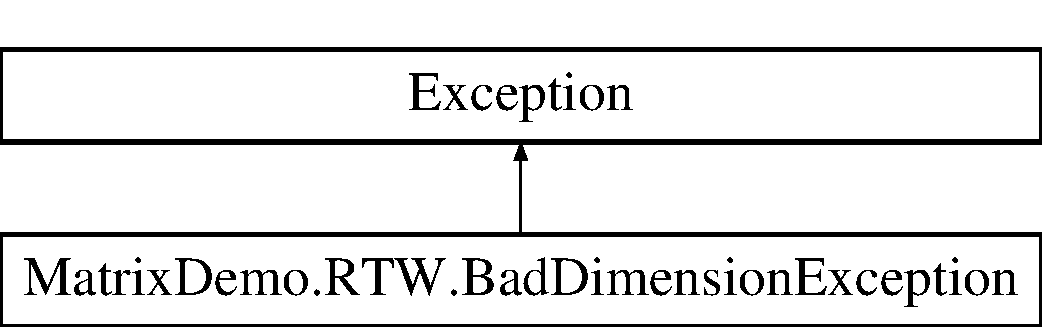
\includegraphics[height=2.000000cm]{class_matrix_demo_1_1_r_t_w_1_1_bad_dimension_exception}
\end{center}
\end{figure}
\subsection*{Public Member Functions}
\begin{DoxyCompactItemize}
\item 
\mbox{\hyperlink{class_matrix_demo_1_1_r_t_w_1_1_bad_dimension_exception_a798ed5eabe99eb0da328d483fc65b872}{Bad\+Dimension\+Exception}} ()
\item 
\mbox{\hyperlink{class_matrix_demo_1_1_r_t_w_1_1_bad_dimension_exception_acb08f6b3204a52bab02d4a2b2bd5018d}{Bad\+Dimension\+Exception}} (String message)
\item 
\mbox{\hyperlink{class_matrix_demo_1_1_r_t_w_1_1_bad_dimension_exception_ac8b77428bbfa83daf5d72873c5ea2cfa}{Bad\+Dimension\+Exception}} (Serialization\+Info sinfo, Streaming\+Context scontext)
\item 
\mbox{\hyperlink{class_matrix_demo_1_1_r_t_w_1_1_bad_dimension_exception_a7cbc7dfbc98f0834b5954db4e41a5c10}{Bad\+Dimension\+Exception}} (String message, Exception ex)
\end{DoxyCompactItemize}


\subsection{Detailed Description}
The \mbox{\hyperlink{class_matrix_demo_1_1_r_t_w_1_1_bad_dimension_exception}{Bad\+Dimension\+Exception}} is thrown when a matrix operation is incompatible with the dimensions of its operands. 



\subsection{Constructor \& Destructor Documentation}
\mbox{\Hypertarget{class_matrix_demo_1_1_r_t_w_1_1_bad_dimension_exception_a798ed5eabe99eb0da328d483fc65b872}\label{class_matrix_demo_1_1_r_t_w_1_1_bad_dimension_exception_a798ed5eabe99eb0da328d483fc65b872}} 
\index{Matrix\+Demo\+::\+R\+T\+W\+::\+Bad\+Dimension\+Exception@{Matrix\+Demo\+::\+R\+T\+W\+::\+Bad\+Dimension\+Exception}!Bad\+Dimension\+Exception@{Bad\+Dimension\+Exception}}
\index{Bad\+Dimension\+Exception@{Bad\+Dimension\+Exception}!Matrix\+Demo\+::\+R\+T\+W\+::\+Bad\+Dimension\+Exception@{Matrix\+Demo\+::\+R\+T\+W\+::\+Bad\+Dimension\+Exception}}
\subsubsection{\texorpdfstring{Bad\+Dimension\+Exception()}{BadDimensionException()}\hspace{0.1cm}{\footnotesize\ttfamily [1/4]}}
{\footnotesize\ttfamily Matrix\+Demo.\+R\+T\+W.\+Bad\+Dimension\+Exception.\+Bad\+Dimension\+Exception (\begin{DoxyParamCaption}{ }\end{DoxyParamCaption})}

\mbox{\Hypertarget{class_matrix_demo_1_1_r_t_w_1_1_bad_dimension_exception_acb08f6b3204a52bab02d4a2b2bd5018d}\label{class_matrix_demo_1_1_r_t_w_1_1_bad_dimension_exception_acb08f6b3204a52bab02d4a2b2bd5018d}} 
\index{Matrix\+Demo\+::\+R\+T\+W\+::\+Bad\+Dimension\+Exception@{Matrix\+Demo\+::\+R\+T\+W\+::\+Bad\+Dimension\+Exception}!Bad\+Dimension\+Exception@{Bad\+Dimension\+Exception}}
\index{Bad\+Dimension\+Exception@{Bad\+Dimension\+Exception}!Matrix\+Demo\+::\+R\+T\+W\+::\+Bad\+Dimension\+Exception@{Matrix\+Demo\+::\+R\+T\+W\+::\+Bad\+Dimension\+Exception}}
\subsubsection{\texorpdfstring{Bad\+Dimension\+Exception()}{BadDimensionException()}\hspace{0.1cm}{\footnotesize\ttfamily [2/4]}}
{\footnotesize\ttfamily Matrix\+Demo.\+R\+T\+W.\+Bad\+Dimension\+Exception.\+Bad\+Dimension\+Exception (\begin{DoxyParamCaption}\item[{String}]{message }\end{DoxyParamCaption})}

\mbox{\Hypertarget{class_matrix_demo_1_1_r_t_w_1_1_bad_dimension_exception_ac8b77428bbfa83daf5d72873c5ea2cfa}\label{class_matrix_demo_1_1_r_t_w_1_1_bad_dimension_exception_ac8b77428bbfa83daf5d72873c5ea2cfa}} 
\index{Matrix\+Demo\+::\+R\+T\+W\+::\+Bad\+Dimension\+Exception@{Matrix\+Demo\+::\+R\+T\+W\+::\+Bad\+Dimension\+Exception}!Bad\+Dimension\+Exception@{Bad\+Dimension\+Exception}}
\index{Bad\+Dimension\+Exception@{Bad\+Dimension\+Exception}!Matrix\+Demo\+::\+R\+T\+W\+::\+Bad\+Dimension\+Exception@{Matrix\+Demo\+::\+R\+T\+W\+::\+Bad\+Dimension\+Exception}}
\subsubsection{\texorpdfstring{Bad\+Dimension\+Exception()}{BadDimensionException()}\hspace{0.1cm}{\footnotesize\ttfamily [3/4]}}
{\footnotesize\ttfamily Matrix\+Demo.\+R\+T\+W.\+Bad\+Dimension\+Exception.\+Bad\+Dimension\+Exception (\begin{DoxyParamCaption}\item[{Serialization\+Info}]{sinfo,  }\item[{Streaming\+Context}]{scontext }\end{DoxyParamCaption})}

\mbox{\Hypertarget{class_matrix_demo_1_1_r_t_w_1_1_bad_dimension_exception_a7cbc7dfbc98f0834b5954db4e41a5c10}\label{class_matrix_demo_1_1_r_t_w_1_1_bad_dimension_exception_a7cbc7dfbc98f0834b5954db4e41a5c10}} 
\index{Matrix\+Demo\+::\+R\+T\+W\+::\+Bad\+Dimension\+Exception@{Matrix\+Demo\+::\+R\+T\+W\+::\+Bad\+Dimension\+Exception}!Bad\+Dimension\+Exception@{Bad\+Dimension\+Exception}}
\index{Bad\+Dimension\+Exception@{Bad\+Dimension\+Exception}!Matrix\+Demo\+::\+R\+T\+W\+::\+Bad\+Dimension\+Exception@{Matrix\+Demo\+::\+R\+T\+W\+::\+Bad\+Dimension\+Exception}}
\subsubsection{\texorpdfstring{Bad\+Dimension\+Exception()}{BadDimensionException()}\hspace{0.1cm}{\footnotesize\ttfamily [4/4]}}
{\footnotesize\ttfamily Matrix\+Demo.\+R\+T\+W.\+Bad\+Dimension\+Exception.\+Bad\+Dimension\+Exception (\begin{DoxyParamCaption}\item[{String}]{message,  }\item[{Exception}]{ex }\end{DoxyParamCaption})}



The documentation for this class was generated from the following file\+:\begin{DoxyCompactItemize}
\item 
C\+:/\+Users/\+Nathann Hohnbaum/\+Source/\+Repos/\+Matrix-\/\+Program/\+Matrix\+Demo/\+Matrix\+Demo/\+R\+T\+W/\mbox{\hyperlink{_bad_dimension_exception_8cs}{Bad\+Dimension\+Exception.\+cs}}\end{DoxyCompactItemize}

\hypertarget{class_matrix_demo_1_1_demo_view}{}\section{Matrix\+Demo.\+Demo\+View Class Reference}
\label{class_matrix_demo_1_1_demo_view}\index{Matrix\+Demo.\+Demo\+View@{Matrix\+Demo.\+Demo\+View}}
Inheritance diagram for Matrix\+Demo.\+Demo\+View\+:\begin{figure}[H]
\begin{center}
\leavevmode
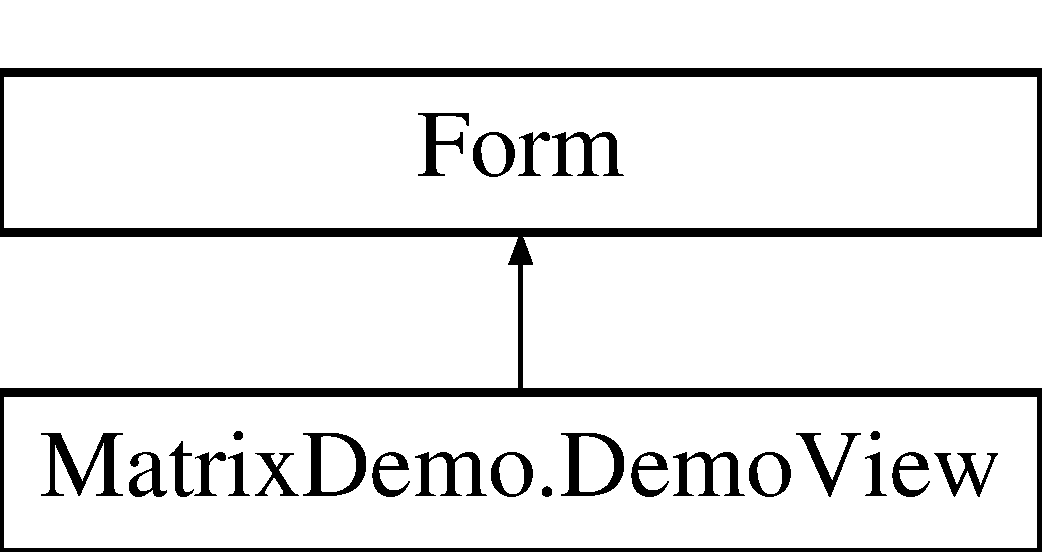
\includegraphics[height=2.000000cm]{class_matrix_demo_1_1_demo_view}
\end{center}
\end{figure}
\subsection*{Public Member Functions}
\begin{DoxyCompactItemize}
\item 
\mbox{\hyperlink{class_matrix_demo_1_1_demo_view_a5ee0e84d6a82ade59b387064eb9e138d}{Demo\+View}} ()
\end{DoxyCompactItemize}
\subsection*{Protected Member Functions}
\begin{DoxyCompactItemize}
\item 
override void \mbox{\hyperlink{class_matrix_demo_1_1_demo_view_a81f680e49d2873816234e512c49f07b7}{Dispose}} (bool disposing)
\begin{DoxyCompactList}\small\item\em Clean up any resources being used. \end{DoxyCompactList}\end{DoxyCompactItemize}


\subsection{Constructor \& Destructor Documentation}
\mbox{\Hypertarget{class_matrix_demo_1_1_demo_view_a5ee0e84d6a82ade59b387064eb9e138d}\label{class_matrix_demo_1_1_demo_view_a5ee0e84d6a82ade59b387064eb9e138d}} 
\index{Matrix\+Demo\+::\+Demo\+View@{Matrix\+Demo\+::\+Demo\+View}!Demo\+View@{Demo\+View}}
\index{Demo\+View@{Demo\+View}!Matrix\+Demo\+::\+Demo\+View@{Matrix\+Demo\+::\+Demo\+View}}
\subsubsection{\texorpdfstring{Demo\+View()}{DemoView()}}
{\footnotesize\ttfamily Matrix\+Demo.\+Demo\+View.\+Demo\+View (\begin{DoxyParamCaption}{ }\end{DoxyParamCaption})}



\subsection{Member Function Documentation}
\mbox{\Hypertarget{class_matrix_demo_1_1_demo_view_a81f680e49d2873816234e512c49f07b7}\label{class_matrix_demo_1_1_demo_view_a81f680e49d2873816234e512c49f07b7}} 
\index{Matrix\+Demo\+::\+Demo\+View@{Matrix\+Demo\+::\+Demo\+View}!Dispose@{Dispose}}
\index{Dispose@{Dispose}!Matrix\+Demo\+::\+Demo\+View@{Matrix\+Demo\+::\+Demo\+View}}
\subsubsection{\texorpdfstring{Dispose()}{Dispose()}}
{\footnotesize\ttfamily override void Matrix\+Demo.\+Demo\+View.\+Dispose (\begin{DoxyParamCaption}\item[{bool}]{disposing }\end{DoxyParamCaption})\hspace{0.3cm}{\ttfamily [protected]}}



Clean up any resources being used. 


\begin{DoxyParams}{Parameters}
{\em disposing} & true if managed resources should be disposed; otherwise, false.\\
\hline
\end{DoxyParams}


The documentation for this class was generated from the following files\+:\begin{DoxyCompactItemize}
\item 
C\+:/\+Users/\+Nathann Hohnbaum/\+Source/\+Repos/\+Matrix-\/\+Program/\+Matrix\+Demo/\+Matrix\+Demo/\mbox{\hyperlink{_demo_view_8cs}{Demo\+View.\+cs}}\item 
C\+:/\+Users/\+Nathann Hohnbaum/\+Source/\+Repos/\+Matrix-\/\+Program/\+Matrix\+Demo/\+Matrix\+Demo/\mbox{\hyperlink{_demo_view_8_designer_8cs}{Demo\+View.\+Designer.\+cs}}\end{DoxyCompactItemize}

\hypertarget{class_matrix_demo_1_1_r_t_w_1_1_matrix}{}\section{Matrix\+Demo.\+R\+T\+W.\+Matrix Class Reference}
\label{class_matrix_demo_1_1_r_t_w_1_1_matrix}\index{Matrix\+Demo.\+R\+T\+W.\+Matrix@{Matrix\+Demo.\+R\+T\+W.\+Matrix}}


The matrix class stores a matrix of doubles. It uses an indexer to access elements and properties for readonly values of rows and columns. It also uses operator overloading to support matrix additoin, matrix subtraction, matrix inversion, scalar multiplication, and matrix multiplication. In addition, it has several methods to perform operations including transposition, reducing to reduced row echelon form, inversion, and computing determinants.  


\subsection*{Public Member Functions}
\begin{DoxyCompactItemize}
\item 
\mbox{\hyperlink{class_matrix_demo_1_1_r_t_w_1_1_matrix_a8c22efc901ad89be3078a180a7ac15d0}{Matrix}} (int rows, int cols)
\begin{DoxyCompactList}\small\item\em Creates a zero matrix with the specified number of rows and columns. \end{DoxyCompactList}\item 
\mbox{\hyperlink{class_matrix_demo_1_1_r_t_w_1_1_matrix_ad2a320fd0c86551f34070679fd43433c}{Matrix}} (double\mbox{[},\mbox{]} e)
\begin{DoxyCompactList}\small\item\em Creates a matrix and populates it with entries from a given array of doubles. The matrix is not backed by the 2-\/dimensional array of doubles, so changes in one will not affect the other. For a \mbox{\hyperlink{class_matrix_demo_1_1_r_t_w_1_1_matrix}{Matrix}} backed by the array of doubles, use \mbox{\hyperlink{class_matrix_demo_1_1_r_t_w_1_1_matrix_a0c737f7e6b54edac4d26b4f1c595ee92}{operator Matrix}}. \end{DoxyCompactList}\item 
double \mbox{[},\mbox{]} \mbox{\hyperlink{class_matrix_demo_1_1_r_t_w_1_1_matrix_a9f6f8e0e7acfbdd55852f258daf68b8f}{Get\+Entries}} ()
\begin{DoxyCompactList}\small\item\em Returns a 2-\/dimensional array of doubles reflecting the entries in the matrix. The resulting 2-\/dimensional array is not backed by the matrix, so changes in one will not affect the other. For a backed 2-\/dimensional array of doubles, use \mbox{\hyperlink{class_matrix_demo_1_1_r_t_w_1_1_matrix_ac23641ac04b3c3baf14174bdf9049db2}{operator double\mbox{[},\mbox{]}}}. \end{DoxyCompactList}\item 
void \mbox{\hyperlink{class_matrix_demo_1_1_r_t_w_1_1_matrix_a14fc1e8ce8136690364961901e7becf6}{Reduce}} ()
\begin{DoxyCompactList}\small\item\em Converts this matrix to Reduced Row Echelon Form. \end{DoxyCompactList}\item 
\mbox{\hyperlink{class_matrix_demo_1_1_r_t_w_1_1_matrix}{Matrix}} \mbox{\hyperlink{class_matrix_demo_1_1_r_t_w_1_1_matrix_ab5b22330a32e73b322522e9c60b8502e}{R\+R\+EF}} ()
\begin{DoxyCompactList}\small\item\em Returns the Reduced Row Echelon form of this matrix. This matrix its4elf is unaltered. \end{DoxyCompactList}\item 
double \mbox{\hyperlink{class_matrix_demo_1_1_r_t_w_1_1_matrix_a1bf322e5e6ff6ae935c74a91df5bb51c}{Determinant}} ()
\begin{DoxyCompactList}\small\item\em Calculates the determinant of this matrix. \end{DoxyCompactList}\item 
\mbox{\hyperlink{class_matrix_demo_1_1_r_t_w_1_1_matrix}{Matrix}} \mbox{\hyperlink{class_matrix_demo_1_1_r_t_w_1_1_matrix_a6d733a0dfeef17bf64c99671bc4cb116}{Inverse}} ()
\begin{DoxyCompactList}\small\item\em Returns the inverse of this matrix if it exists. \end{DoxyCompactList}\item 
\mbox{\hyperlink{class_matrix_demo_1_1_r_t_w_1_1_matrix}{Matrix}} \mbox{\hyperlink{class_matrix_demo_1_1_r_t_w_1_1_matrix_a2718067191d516f881e29baf49db7604}{Transpose}} ()
\begin{DoxyCompactList}\small\item\em Returns the tramspose of this matrix. \end{DoxyCompactList}\item 
override string \mbox{\hyperlink{class_matrix_demo_1_1_r_t_w_1_1_matrix_a6dcaf1d6a6050cea143f68da4a802900}{To\+String}} ()
\begin{DoxyCompactList}\small\item\em Returns a String representation of this matrix. \end{DoxyCompactList}\item 
override int \mbox{\hyperlink{class_matrix_demo_1_1_r_t_w_1_1_matrix_ad7f43b0fc8f78f4deb76238d99749d1d}{Get\+Hash\+Code}} ()
\begin{DoxyCompactList}\small\item\em Returns the hash code for this matrix. \end{DoxyCompactList}\item 
override bool \mbox{\hyperlink{class_matrix_demo_1_1_r_t_w_1_1_matrix_ac0f3f4cf1a7f5d36aff55a94d7ae6c92}{Equals}} (object obj)
\begin{DoxyCompactList}\small\item\em Returns true if this matrix is equal to the other matrix. \end{DoxyCompactList}\end{DoxyCompactItemize}
\subsection*{Static Public Member Functions}
\begin{DoxyCompactItemize}
\item 
static implicit \mbox{\hyperlink{class_matrix_demo_1_1_r_t_w_1_1_matrix_ac23641ac04b3c3baf14174bdf9049db2}{operator double\mbox{[},\mbox{]}}} (\mbox{\hyperlink{class_matrix_demo_1_1_r_t_w_1_1_matrix}{Matrix}} m)
\begin{DoxyCompactList}\small\item\em Converts a \mbox{\hyperlink{class_matrix_demo_1_1_r_t_w_1_1_matrix}{Matrix}} to a 2-\/dimensional array of doubles. The resulting 2-\/dimensional array is backed by the matrix, so changes in one will affect the other. For a 2-\/dimensional array of entries not backed by the matrix, use \mbox{\hyperlink{class_matrix_demo_1_1_r_t_w_1_1_matrix_a9f6f8e0e7acfbdd55852f258daf68b8f}{Get\+Entries}}. \end{DoxyCompactList}\item 
static implicit \mbox{\hyperlink{class_matrix_demo_1_1_r_t_w_1_1_matrix_a0c737f7e6b54edac4d26b4f1c595ee92}{operator Matrix}} (double\mbox{[},\mbox{]} e)
\begin{DoxyCompactList}\small\item\em Converts a 2-\/dimensional array of doubles to a matrix. The resulting matrix is backed by the array, so changes in one will affect the other. For a \mbox{\hyperlink{class_matrix_demo_1_1_r_t_w_1_1_matrix}{Matrix}} not backed by the 2-\/dimensional array of entries, use \mbox{\hyperlink{class_matrix_demo_1_1_r_t_w_1_1_matrix_ad2a320fd0c86551f34070679fd43433c}{Matrix.\+Matrix(double\mbox{[},\mbox{]})}}. \end{DoxyCompactList}\item 
static \mbox{\hyperlink{class_matrix_demo_1_1_r_t_w_1_1_matrix}{Matrix}} \mbox{\hyperlink{class_matrix_demo_1_1_r_t_w_1_1_matrix_a6c0787446dfff85088742793f129729a}{operator+}} (\mbox{\hyperlink{class_matrix_demo_1_1_r_t_w_1_1_matrix}{Matrix}} lhs, \mbox{\hyperlink{class_matrix_demo_1_1_r_t_w_1_1_matrix}{Matrix}} rhs)
\begin{DoxyCompactList}\small\item\em Returns the matrix sum of the two matrices. \end{DoxyCompactList}\item 
static \mbox{\hyperlink{class_matrix_demo_1_1_r_t_w_1_1_matrix}{Matrix}} \mbox{\hyperlink{class_matrix_demo_1_1_r_t_w_1_1_matrix_a7d96c0cc84a8ae412014464007fbb576}{operator-\/}} (\mbox{\hyperlink{class_matrix_demo_1_1_r_t_w_1_1_matrix}{Matrix}} lhs, \mbox{\hyperlink{class_matrix_demo_1_1_r_t_w_1_1_matrix}{Matrix}} rhs)
\begin{DoxyCompactList}\small\item\em Returns the matrix difference of the two matrices. \end{DoxyCompactList}\item 
static \mbox{\hyperlink{class_matrix_demo_1_1_r_t_w_1_1_matrix}{Matrix}} \mbox{\hyperlink{class_matrix_demo_1_1_r_t_w_1_1_matrix_a115c01ce2236a801cfa99bb685aea0ff}{operator-\/}} (\mbox{\hyperlink{class_matrix_demo_1_1_r_t_w_1_1_matrix}{Matrix}} m)
\begin{DoxyCompactList}\small\item\em Takes the opposite of the given matrix. \end{DoxyCompactList}\item 
static \mbox{\hyperlink{class_matrix_demo_1_1_r_t_w_1_1_matrix}{Matrix}} \mbox{\hyperlink{class_matrix_demo_1_1_r_t_w_1_1_matrix_ae315e38f4441e1df65dd5226b55314ea}{operator$\ast$}} (double s, \mbox{\hyperlink{class_matrix_demo_1_1_r_t_w_1_1_matrix}{Matrix}} m)
\begin{DoxyCompactList}\small\item\em Scales a matrix by a scalar. \end{DoxyCompactList}\item 
static \mbox{\hyperlink{class_matrix_demo_1_1_r_t_w_1_1_matrix}{Matrix}} \mbox{\hyperlink{class_matrix_demo_1_1_r_t_w_1_1_matrix_a5d72530d3d2ddc47341e82ec1a076b71}{operator$\ast$}} (\mbox{\hyperlink{class_matrix_demo_1_1_r_t_w_1_1_matrix}{Matrix}} lhs, \mbox{\hyperlink{class_matrix_demo_1_1_r_t_w_1_1_matrix}{Matrix}} rhs)
\begin{DoxyCompactList}\small\item\em Performs matrix multiplication. \end{DoxyCompactList}\end{DoxyCompactItemize}
\subsection*{Properties}
\begin{DoxyCompactItemize}
\item 
int \mbox{\hyperlink{class_matrix_demo_1_1_r_t_w_1_1_matrix_a9596bae43484cf8c21729237297b4744}{Rows}}\hspace{0.3cm}{\ttfamily  \mbox{[}get\mbox{]}}
\begin{DoxyCompactList}\small\item\em The number of rows in the matrix \end{DoxyCompactList}\item 
int \mbox{\hyperlink{class_matrix_demo_1_1_r_t_w_1_1_matrix_a7b412909ff1b6c6b9c9af57314dff52b}{Cols}}\hspace{0.3cm}{\ttfamily  \mbox{[}get\mbox{]}}
\begin{DoxyCompactList}\small\item\em The number of columns in the matrix \end{DoxyCompactList}\item 
double \mbox{\hyperlink{class_matrix_demo_1_1_r_t_w_1_1_matrix_aa908f44fc8fd669347ba6a4833406f66}{this\mbox{[}int row, int col\mbox{]}}}\hspace{0.3cm}{\ttfamily  \mbox{[}get, set\mbox{]}}
\begin{DoxyCompactList}\small\item\em Accesses a specific entry in the matrix. \end{DoxyCompactList}\end{DoxyCompactItemize}


\subsection{Detailed Description}
The matrix class stores a matrix of doubles. It uses an indexer to access elements and properties for readonly values of rows and columns. It also uses operator overloading to support matrix additoin, matrix subtraction, matrix inversion, scalar multiplication, and matrix multiplication. In addition, it has several methods to perform operations including transposition, reducing to reduced row echelon form, inversion, and computing determinants. 



\subsection{Constructor \& Destructor Documentation}
\mbox{\Hypertarget{class_matrix_demo_1_1_r_t_w_1_1_matrix_a8c22efc901ad89be3078a180a7ac15d0}\label{class_matrix_demo_1_1_r_t_w_1_1_matrix_a8c22efc901ad89be3078a180a7ac15d0}} 
\index{Matrix\+Demo\+::\+R\+T\+W\+::\+Matrix@{Matrix\+Demo\+::\+R\+T\+W\+::\+Matrix}!Matrix@{Matrix}}
\index{Matrix@{Matrix}!Matrix\+Demo\+::\+R\+T\+W\+::\+Matrix@{Matrix\+Demo\+::\+R\+T\+W\+::\+Matrix}}
\subsubsection{\texorpdfstring{Matrix()}{Matrix()}\hspace{0.1cm}{\footnotesize\ttfamily [1/2]}}
{\footnotesize\ttfamily Matrix\+Demo.\+R\+T\+W.\+Matrix.\+Matrix (\begin{DoxyParamCaption}\item[{int}]{rows,  }\item[{int}]{cols }\end{DoxyParamCaption})}



Creates a zero matrix with the specified number of rows and columns. 


\begin{DoxyParams}{Parameters}
{\em rows} & the number of rows for the matrix.\\
\hline
{\em cols} & the number of columns for the matrix.\\
\hline
\end{DoxyParams}

\begin{DoxyExceptions}{Exceptions}
{\em Argument\+Exception} & Thrown if either or both of the dimensions is negative.\\
\hline
\end{DoxyExceptions}
\mbox{\Hypertarget{class_matrix_demo_1_1_r_t_w_1_1_matrix_ad2a320fd0c86551f34070679fd43433c}\label{class_matrix_demo_1_1_r_t_w_1_1_matrix_ad2a320fd0c86551f34070679fd43433c}} 
\index{Matrix\+Demo\+::\+R\+T\+W\+::\+Matrix@{Matrix\+Demo\+::\+R\+T\+W\+::\+Matrix}!Matrix@{Matrix}}
\index{Matrix@{Matrix}!Matrix\+Demo\+::\+R\+T\+W\+::\+Matrix@{Matrix\+Demo\+::\+R\+T\+W\+::\+Matrix}}
\subsubsection{\texorpdfstring{Matrix()}{Matrix()}\hspace{0.1cm}{\footnotesize\ttfamily [2/2]}}
{\footnotesize\ttfamily Matrix\+Demo.\+R\+T\+W.\+Matrix.\+Matrix (\begin{DoxyParamCaption}\item[{double}]{e\mbox{[},\mbox{]} }\end{DoxyParamCaption})}



Creates a matrix and populates it with entries from a given array of doubles. The matrix is not backed by the 2-\/dimensional array of doubles, so changes in one will not affect the other. For a \mbox{\hyperlink{class_matrix_demo_1_1_r_t_w_1_1_matrix}{Matrix}} backed by the array of doubles, use \mbox{\hyperlink{class_matrix_demo_1_1_r_t_w_1_1_matrix_a0c737f7e6b54edac4d26b4f1c595ee92}{operator Matrix}}. 


\begin{DoxyParams}{Parameters}
{\em e} & The entries to use to populate the matrix.\\
\hline
\end{DoxyParams}
\begin{DoxySeeAlso}{See also}
\mbox{\hyperlink{class_matrix_demo_1_1_r_t_w_1_1_matrix_a0c737f7e6b54edac4d26b4f1c595ee92}{operator Matrix}}


\end{DoxySeeAlso}


\subsection{Member Function Documentation}
\mbox{\Hypertarget{class_matrix_demo_1_1_r_t_w_1_1_matrix_a1bf322e5e6ff6ae935c74a91df5bb51c}\label{class_matrix_demo_1_1_r_t_w_1_1_matrix_a1bf322e5e6ff6ae935c74a91df5bb51c}} 
\index{Matrix\+Demo\+::\+R\+T\+W\+::\+Matrix@{Matrix\+Demo\+::\+R\+T\+W\+::\+Matrix}!Determinant@{Determinant}}
\index{Determinant@{Determinant}!Matrix\+Demo\+::\+R\+T\+W\+::\+Matrix@{Matrix\+Demo\+::\+R\+T\+W\+::\+Matrix}}
\subsubsection{\texorpdfstring{Determinant()}{Determinant()}}
{\footnotesize\ttfamily double Matrix\+Demo.\+R\+T\+W.\+Matrix.\+Determinant (\begin{DoxyParamCaption}{ }\end{DoxyParamCaption})}



Calculates the determinant of this matrix. 

\begin{DoxyReturn}{Returns}
the determinant of this matrix.
\end{DoxyReturn}

\begin{DoxyExceptions}{Exceptions}
{\em \mbox{\hyperlink{class_matrix_demo_1_1_r_t_w_1_1_bad_dimension_exception}{Bad\+Dimension\+Exception}}} & Thrown when the matrix is not square.\\
\hline
\end{DoxyExceptions}
\mbox{\Hypertarget{class_matrix_demo_1_1_r_t_w_1_1_matrix_ac0f3f4cf1a7f5d36aff55a94d7ae6c92}\label{class_matrix_demo_1_1_r_t_w_1_1_matrix_ac0f3f4cf1a7f5d36aff55a94d7ae6c92}} 
\index{Matrix\+Demo\+::\+R\+T\+W\+::\+Matrix@{Matrix\+Demo\+::\+R\+T\+W\+::\+Matrix}!Equals@{Equals}}
\index{Equals@{Equals}!Matrix\+Demo\+::\+R\+T\+W\+::\+Matrix@{Matrix\+Demo\+::\+R\+T\+W\+::\+Matrix}}
\subsubsection{\texorpdfstring{Equals()}{Equals()}}
{\footnotesize\ttfamily override bool Matrix\+Demo.\+R\+T\+W.\+Matrix.\+Equals (\begin{DoxyParamCaption}\item[{object}]{obj }\end{DoxyParamCaption})}



Returns true if this matrix is equal to the other matrix. 


\begin{DoxyParams}{Parameters}
{\em obj} & The object to compare to this matrix.\\
\hline
\end{DoxyParams}
\begin{DoxyReturn}{Returns}
True if the objects are equal, false otherwise.
\end{DoxyReturn}
\mbox{\Hypertarget{class_matrix_demo_1_1_r_t_w_1_1_matrix_a9f6f8e0e7acfbdd55852f258daf68b8f}\label{class_matrix_demo_1_1_r_t_w_1_1_matrix_a9f6f8e0e7acfbdd55852f258daf68b8f}} 
\index{Matrix\+Demo\+::\+R\+T\+W\+::\+Matrix@{Matrix\+Demo\+::\+R\+T\+W\+::\+Matrix}!Get\+Entries@{Get\+Entries}}
\index{Get\+Entries@{Get\+Entries}!Matrix\+Demo\+::\+R\+T\+W\+::\+Matrix@{Matrix\+Demo\+::\+R\+T\+W\+::\+Matrix}}
\subsubsection{\texorpdfstring{Get\+Entries()}{GetEntries()}}
{\footnotesize\ttfamily double \mbox{[},\mbox{]} Matrix\+Demo.\+R\+T\+W.\+Matrix.\+Get\+Entries (\begin{DoxyParamCaption}{ }\end{DoxyParamCaption})}



Returns a 2-\/dimensional array of doubles reflecting the entries in the matrix. The resulting 2-\/dimensional array is not backed by the matrix, so changes in one will not affect the other. For a backed 2-\/dimensional array of doubles, use \mbox{\hyperlink{class_matrix_demo_1_1_r_t_w_1_1_matrix_ac23641ac04b3c3baf14174bdf9049db2}{operator double\mbox{[},\mbox{]}}}. 

\begin{DoxyReturn}{Returns}
A copy of the entries of the \mbox{\hyperlink{class_matrix_demo_1_1_r_t_w_1_1_matrix}{Matrix}}.
\end{DoxyReturn}
\begin{DoxySeeAlso}{See also}
\mbox{\hyperlink{class_matrix_demo_1_1_r_t_w_1_1_matrix_ac23641ac04b3c3baf14174bdf9049db2}{operator double\mbox{[},\mbox{]}}}


\end{DoxySeeAlso}
\mbox{\Hypertarget{class_matrix_demo_1_1_r_t_w_1_1_matrix_ad7f43b0fc8f78f4deb76238d99749d1d}\label{class_matrix_demo_1_1_r_t_w_1_1_matrix_ad7f43b0fc8f78f4deb76238d99749d1d}} 
\index{Matrix\+Demo\+::\+R\+T\+W\+::\+Matrix@{Matrix\+Demo\+::\+R\+T\+W\+::\+Matrix}!Get\+Hash\+Code@{Get\+Hash\+Code}}
\index{Get\+Hash\+Code@{Get\+Hash\+Code}!Matrix\+Demo\+::\+R\+T\+W\+::\+Matrix@{Matrix\+Demo\+::\+R\+T\+W\+::\+Matrix}}
\subsubsection{\texorpdfstring{Get\+Hash\+Code()}{GetHashCode()}}
{\footnotesize\ttfamily override int Matrix\+Demo.\+R\+T\+W.\+Matrix.\+Get\+Hash\+Code (\begin{DoxyParamCaption}{ }\end{DoxyParamCaption})}



Returns the hash code for this matrix. 

\begin{DoxyReturn}{Returns}
The hash code used for hashmaps. $<$note type=\char`\"{}warning\char`\"{}$>$This hash function is not cryptographically secure.$<$/note$>$
\end{DoxyReturn}
\mbox{\Hypertarget{class_matrix_demo_1_1_r_t_w_1_1_matrix_a6d733a0dfeef17bf64c99671bc4cb116}\label{class_matrix_demo_1_1_r_t_w_1_1_matrix_a6d733a0dfeef17bf64c99671bc4cb116}} 
\index{Matrix\+Demo\+::\+R\+T\+W\+::\+Matrix@{Matrix\+Demo\+::\+R\+T\+W\+::\+Matrix}!Inverse@{Inverse}}
\index{Inverse@{Inverse}!Matrix\+Demo\+::\+R\+T\+W\+::\+Matrix@{Matrix\+Demo\+::\+R\+T\+W\+::\+Matrix}}
\subsubsection{\texorpdfstring{Inverse()}{Inverse()}}
{\footnotesize\ttfamily \mbox{\hyperlink{class_matrix_demo_1_1_r_t_w_1_1_matrix}{Matrix}} Matrix\+Demo.\+R\+T\+W.\+Matrix.\+Inverse (\begin{DoxyParamCaption}{ }\end{DoxyParamCaption})}



Returns the inverse of this matrix if it exists. 

\begin{DoxyReturn}{Returns}
Returns the inverse of this matrix if it exists, null otherwise.
\end{DoxyReturn}

\begin{DoxyExceptions}{Exceptions}
{\em \mbox{\hyperlink{class_matrix_demo_1_1_r_t_w_1_1_bad_dimension_exception}{Bad\+Dimension\+Exception}}} & Thrown when the matrix is not square.\\
\hline
\end{DoxyExceptions}
\mbox{\Hypertarget{class_matrix_demo_1_1_r_t_w_1_1_matrix_ac23641ac04b3c3baf14174bdf9049db2}\label{class_matrix_demo_1_1_r_t_w_1_1_matrix_ac23641ac04b3c3baf14174bdf9049db2}} 
\index{Matrix\+Demo\+::\+R\+T\+W\+::\+Matrix@{Matrix\+Demo\+::\+R\+T\+W\+::\+Matrix}!operator double\mbox{[},\mbox{]}@{operator double[,]}}
\index{operator double\mbox{[},\mbox{]}@{operator double[,]}!Matrix\+Demo\+::\+R\+T\+W\+::\+Matrix@{Matrix\+Demo\+::\+R\+T\+W\+::\+Matrix}}
\subsubsection{\texorpdfstring{operator double[,]()}{operator double[,]()}}
{\footnotesize\ttfamily static implicit Matrix\+Demo.\+R\+T\+W.\+Matrix.\+operator double\mbox{[},\mbox{]} (\begin{DoxyParamCaption}\item[{\mbox{\hyperlink{class_matrix_demo_1_1_r_t_w_1_1_matrix}{Matrix}}}]{m }\end{DoxyParamCaption})\hspace{0.3cm}{\ttfamily [static]}}



Converts a \mbox{\hyperlink{class_matrix_demo_1_1_r_t_w_1_1_matrix}{Matrix}} to a 2-\/dimensional array of doubles. The resulting 2-\/dimensional array is backed by the matrix, so changes in one will affect the other. For a 2-\/dimensional array of entries not backed by the matrix, use \mbox{\hyperlink{class_matrix_demo_1_1_r_t_w_1_1_matrix_a9f6f8e0e7acfbdd55852f258daf68b8f}{Get\+Entries}}. 


\begin{DoxyParams}{Parameters}
{\em m} & the matrix to convert.\\
\hline
\end{DoxyParams}
\begin{DoxySeeAlso}{See also}
\mbox{\hyperlink{class_matrix_demo_1_1_r_t_w_1_1_matrix_a9f6f8e0e7acfbdd55852f258daf68b8f}{Get\+Entries}}


\end{DoxySeeAlso}
\mbox{\Hypertarget{class_matrix_demo_1_1_r_t_w_1_1_matrix_a0c737f7e6b54edac4d26b4f1c595ee92}\label{class_matrix_demo_1_1_r_t_w_1_1_matrix_a0c737f7e6b54edac4d26b4f1c595ee92}} 
\index{Matrix\+Demo\+::\+R\+T\+W\+::\+Matrix@{Matrix\+Demo\+::\+R\+T\+W\+::\+Matrix}!operator Matrix@{operator Matrix}}
\index{operator Matrix@{operator Matrix}!Matrix\+Demo\+::\+R\+T\+W\+::\+Matrix@{Matrix\+Demo\+::\+R\+T\+W\+::\+Matrix}}
\subsubsection{\texorpdfstring{operator Matrix()}{operator Matrix()}}
{\footnotesize\ttfamily static implicit Matrix\+Demo.\+R\+T\+W.\+Matrix.\+operator \mbox{\hyperlink{class_matrix_demo_1_1_r_t_w_1_1_matrix}{Matrix}} (\begin{DoxyParamCaption}\item[{double}]{e\mbox{[},\mbox{]} }\end{DoxyParamCaption})\hspace{0.3cm}{\ttfamily [static]}}



Converts a 2-\/dimensional array of doubles to a matrix. The resulting matrix is backed by the array, so changes in one will affect the other. For a \mbox{\hyperlink{class_matrix_demo_1_1_r_t_w_1_1_matrix}{Matrix}} not backed by the 2-\/dimensional array of entries, use \mbox{\hyperlink{class_matrix_demo_1_1_r_t_w_1_1_matrix_ad2a320fd0c86551f34070679fd43433c}{Matrix.\+Matrix(double\mbox{[},\mbox{]})}}. 


\begin{DoxyParams}{Parameters}
{\em e} & The 2-\/dimensional array of doubles to convert.\\
\hline
\end{DoxyParams}
\begin{DoxySeeAlso}{See also}
\mbox{\hyperlink{class_matrix_demo_1_1_r_t_w_1_1_matrix_ad2a320fd0c86551f34070679fd43433c}{Matrix.\+Matrix(double\mbox{[},\mbox{]})}}


\end{DoxySeeAlso}
\mbox{\Hypertarget{class_matrix_demo_1_1_r_t_w_1_1_matrix_ae315e38f4441e1df65dd5226b55314ea}\label{class_matrix_demo_1_1_r_t_w_1_1_matrix_ae315e38f4441e1df65dd5226b55314ea}} 
\index{Matrix\+Demo\+::\+R\+T\+W\+::\+Matrix@{Matrix\+Demo\+::\+R\+T\+W\+::\+Matrix}!operator$\ast$@{operator$\ast$}}
\index{operator$\ast$@{operator$\ast$}!Matrix\+Demo\+::\+R\+T\+W\+::\+Matrix@{Matrix\+Demo\+::\+R\+T\+W\+::\+Matrix}}
\subsubsection{\texorpdfstring{operator$\ast$()}{operator*()}\hspace{0.1cm}{\footnotesize\ttfamily [1/2]}}
{\footnotesize\ttfamily static \mbox{\hyperlink{class_matrix_demo_1_1_r_t_w_1_1_matrix}{Matrix}} Matrix\+Demo.\+R\+T\+W.\+Matrix.\+operator$\ast$ (\begin{DoxyParamCaption}\item[{double}]{s,  }\item[{\mbox{\hyperlink{class_matrix_demo_1_1_r_t_w_1_1_matrix}{Matrix}}}]{m }\end{DoxyParamCaption})\hspace{0.3cm}{\ttfamily [static]}}



Scales a matrix by a scalar. 


\begin{DoxyParams}{Parameters}
{\em s} & The scalar by which to scale the matrix.\\
\hline
{\em m} & The matrix to be scaled.\\
\hline
\end{DoxyParams}
\begin{DoxyReturn}{Returns}
A matrix containing each entry in {\ttfamily m} scaled by {\ttfamily s}.
\end{DoxyReturn}
\mbox{\Hypertarget{class_matrix_demo_1_1_r_t_w_1_1_matrix_a5d72530d3d2ddc47341e82ec1a076b71}\label{class_matrix_demo_1_1_r_t_w_1_1_matrix_a5d72530d3d2ddc47341e82ec1a076b71}} 
\index{Matrix\+Demo\+::\+R\+T\+W\+::\+Matrix@{Matrix\+Demo\+::\+R\+T\+W\+::\+Matrix}!operator$\ast$@{operator$\ast$}}
\index{operator$\ast$@{operator$\ast$}!Matrix\+Demo\+::\+R\+T\+W\+::\+Matrix@{Matrix\+Demo\+::\+R\+T\+W\+::\+Matrix}}
\subsubsection{\texorpdfstring{operator$\ast$()}{operator*()}\hspace{0.1cm}{\footnotesize\ttfamily [2/2]}}
{\footnotesize\ttfamily static \mbox{\hyperlink{class_matrix_demo_1_1_r_t_w_1_1_matrix}{Matrix}} Matrix\+Demo.\+R\+T\+W.\+Matrix.\+operator$\ast$ (\begin{DoxyParamCaption}\item[{\mbox{\hyperlink{class_matrix_demo_1_1_r_t_w_1_1_matrix}{Matrix}}}]{lhs,  }\item[{\mbox{\hyperlink{class_matrix_demo_1_1_r_t_w_1_1_matrix}{Matrix}}}]{rhs }\end{DoxyParamCaption})\hspace{0.3cm}{\ttfamily [static]}}



Performs matrix multiplication. 


\begin{DoxyParams}{Parameters}
{\em lhs} & The left hand side of the multiplication.\\
\hline
{\em rhs} & The right hand side of the multiplication.\\
\hline
\end{DoxyParams}
\begin{DoxyReturn}{Returns}
The product of the two matrices.
\end{DoxyReturn}

\begin{DoxyExceptions}{Exceptions}
{\em \mbox{\hyperlink{class_matrix_demo_1_1_r_t_w_1_1_bad_dimension_exception}{Bad\+Dimension\+Exception}}} & Thrown if the number of columns in the left hand side is different from the number of rows in the right hand side.\\
\hline
\end{DoxyExceptions}
\mbox{\Hypertarget{class_matrix_demo_1_1_r_t_w_1_1_matrix_a6c0787446dfff85088742793f129729a}\label{class_matrix_demo_1_1_r_t_w_1_1_matrix_a6c0787446dfff85088742793f129729a}} 
\index{Matrix\+Demo\+::\+R\+T\+W\+::\+Matrix@{Matrix\+Demo\+::\+R\+T\+W\+::\+Matrix}!operator+@{operator+}}
\index{operator+@{operator+}!Matrix\+Demo\+::\+R\+T\+W\+::\+Matrix@{Matrix\+Demo\+::\+R\+T\+W\+::\+Matrix}}
\subsubsection{\texorpdfstring{operator+()}{operator+()}}
{\footnotesize\ttfamily static \mbox{\hyperlink{class_matrix_demo_1_1_r_t_w_1_1_matrix}{Matrix}} Matrix\+Demo.\+R\+T\+W.\+Matrix.\+operator+ (\begin{DoxyParamCaption}\item[{\mbox{\hyperlink{class_matrix_demo_1_1_r_t_w_1_1_matrix}{Matrix}}}]{lhs,  }\item[{\mbox{\hyperlink{class_matrix_demo_1_1_r_t_w_1_1_matrix}{Matrix}}}]{rhs }\end{DoxyParamCaption})\hspace{0.3cm}{\ttfamily [static]}}



Returns the matrix sum of the two matrices. 


\begin{DoxyParams}{Parameters}
{\em lhs} & The left hand side of the addition.\\
\hline
{\em rhs} & The right hand side of the addition.\\
\hline
\end{DoxyParams}
\begin{DoxyReturn}{Returns}
The sum of the two matrices.
\end{DoxyReturn}

\begin{DoxyExceptions}{Exceptions}
{\em \mbox{\hyperlink{class_matrix_demo_1_1_r_t_w_1_1_bad_dimension_exception}{Bad\+Dimension\+Exception}}} & Thrown when the two matrices are of different dimensions.\\
\hline
\end{DoxyExceptions}
\mbox{\Hypertarget{class_matrix_demo_1_1_r_t_w_1_1_matrix_a7d96c0cc84a8ae412014464007fbb576}\label{class_matrix_demo_1_1_r_t_w_1_1_matrix_a7d96c0cc84a8ae412014464007fbb576}} 
\index{Matrix\+Demo\+::\+R\+T\+W\+::\+Matrix@{Matrix\+Demo\+::\+R\+T\+W\+::\+Matrix}!operator-\/@{operator-\/}}
\index{operator-\/@{operator-\/}!Matrix\+Demo\+::\+R\+T\+W\+::\+Matrix@{Matrix\+Demo\+::\+R\+T\+W\+::\+Matrix}}
\subsubsection{\texorpdfstring{operator-\/()}{operator-()}\hspace{0.1cm}{\footnotesize\ttfamily [1/2]}}
{\footnotesize\ttfamily static \mbox{\hyperlink{class_matrix_demo_1_1_r_t_w_1_1_matrix}{Matrix}} Matrix\+Demo.\+R\+T\+W.\+Matrix.\+operator-\/ (\begin{DoxyParamCaption}\item[{\mbox{\hyperlink{class_matrix_demo_1_1_r_t_w_1_1_matrix}{Matrix}}}]{lhs,  }\item[{\mbox{\hyperlink{class_matrix_demo_1_1_r_t_w_1_1_matrix}{Matrix}}}]{rhs }\end{DoxyParamCaption})\hspace{0.3cm}{\ttfamily [static]}}



Returns the matrix difference of the two matrices. 


\begin{DoxyParams}{Parameters}
{\em lhs} & The left hand side of the subtraction.\\
\hline
{\em rhs} & The right hand side of the subtraction.\\
\hline
\end{DoxyParams}
\begin{DoxyReturn}{Returns}
The difference of the two matrices.
\end{DoxyReturn}

\begin{DoxyExceptions}{Exceptions}
{\em \mbox{\hyperlink{class_matrix_demo_1_1_r_t_w_1_1_bad_dimension_exception}{Bad\+Dimension\+Exception}}} & Thrown when the two matrices are of different dimensions.\\
\hline
\end{DoxyExceptions}
\mbox{\Hypertarget{class_matrix_demo_1_1_r_t_w_1_1_matrix_a115c01ce2236a801cfa99bb685aea0ff}\label{class_matrix_demo_1_1_r_t_w_1_1_matrix_a115c01ce2236a801cfa99bb685aea0ff}} 
\index{Matrix\+Demo\+::\+R\+T\+W\+::\+Matrix@{Matrix\+Demo\+::\+R\+T\+W\+::\+Matrix}!operator-\/@{operator-\/}}
\index{operator-\/@{operator-\/}!Matrix\+Demo\+::\+R\+T\+W\+::\+Matrix@{Matrix\+Demo\+::\+R\+T\+W\+::\+Matrix}}
\subsubsection{\texorpdfstring{operator-\/()}{operator-()}\hspace{0.1cm}{\footnotesize\ttfamily [2/2]}}
{\footnotesize\ttfamily static \mbox{\hyperlink{class_matrix_demo_1_1_r_t_w_1_1_matrix}{Matrix}} Matrix\+Demo.\+R\+T\+W.\+Matrix.\+operator-\/ (\begin{DoxyParamCaption}\item[{\mbox{\hyperlink{class_matrix_demo_1_1_r_t_w_1_1_matrix}{Matrix}}}]{m }\end{DoxyParamCaption})\hspace{0.3cm}{\ttfamily [static]}}



Takes the opposite of the given matrix. 


\begin{DoxyParams}{Parameters}
{\em m} & The \mbox{\hyperlink{class_matrix_demo_1_1_r_t_w_1_1_matrix}{Matrix}} to find the opposite of.\\
\hline
\end{DoxyParams}
\begin{DoxyReturn}{Returns}
The opposite of the given matrix. Subtracting {\ttfamily m} from another matrix is equivalent to adding {\ttfamily -\/m} to it.
\end{DoxyReturn}
\mbox{\Hypertarget{class_matrix_demo_1_1_r_t_w_1_1_matrix_a14fc1e8ce8136690364961901e7becf6}\label{class_matrix_demo_1_1_r_t_w_1_1_matrix_a14fc1e8ce8136690364961901e7becf6}} 
\index{Matrix\+Demo\+::\+R\+T\+W\+::\+Matrix@{Matrix\+Demo\+::\+R\+T\+W\+::\+Matrix}!Reduce@{Reduce}}
\index{Reduce@{Reduce}!Matrix\+Demo\+::\+R\+T\+W\+::\+Matrix@{Matrix\+Demo\+::\+R\+T\+W\+::\+Matrix}}
\subsubsection{\texorpdfstring{Reduce()}{Reduce()}}
{\footnotesize\ttfamily void Matrix\+Demo.\+R\+T\+W.\+Matrix.\+Reduce (\begin{DoxyParamCaption}{ }\end{DoxyParamCaption})}



Converts this matrix to Reduced Row Echelon Form. 

\mbox{\Hypertarget{class_matrix_demo_1_1_r_t_w_1_1_matrix_ab5b22330a32e73b322522e9c60b8502e}\label{class_matrix_demo_1_1_r_t_w_1_1_matrix_ab5b22330a32e73b322522e9c60b8502e}} 
\index{Matrix\+Demo\+::\+R\+T\+W\+::\+Matrix@{Matrix\+Demo\+::\+R\+T\+W\+::\+Matrix}!R\+R\+EF@{R\+R\+EF}}
\index{R\+R\+EF@{R\+R\+EF}!Matrix\+Demo\+::\+R\+T\+W\+::\+Matrix@{Matrix\+Demo\+::\+R\+T\+W\+::\+Matrix}}
\subsubsection{\texorpdfstring{R\+R\+E\+F()}{RREF()}}
{\footnotesize\ttfamily \mbox{\hyperlink{class_matrix_demo_1_1_r_t_w_1_1_matrix}{Matrix}} Matrix\+Demo.\+R\+T\+W.\+Matrix.\+R\+R\+EF (\begin{DoxyParamCaption}{ }\end{DoxyParamCaption})}



Returns the Reduced Row Echelon form of this matrix. This matrix its4elf is unaltered. 

\begin{DoxyReturn}{Returns}
the reduced row echelon form of this matrix.
\end{DoxyReturn}
\mbox{\Hypertarget{class_matrix_demo_1_1_r_t_w_1_1_matrix_a6dcaf1d6a6050cea143f68da4a802900}\label{class_matrix_demo_1_1_r_t_w_1_1_matrix_a6dcaf1d6a6050cea143f68da4a802900}} 
\index{Matrix\+Demo\+::\+R\+T\+W\+::\+Matrix@{Matrix\+Demo\+::\+R\+T\+W\+::\+Matrix}!To\+String@{To\+String}}
\index{To\+String@{To\+String}!Matrix\+Demo\+::\+R\+T\+W\+::\+Matrix@{Matrix\+Demo\+::\+R\+T\+W\+::\+Matrix}}
\subsubsection{\texorpdfstring{To\+String()}{ToString()}}
{\footnotesize\ttfamily override string Matrix\+Demo.\+R\+T\+W.\+Matrix.\+To\+String (\begin{DoxyParamCaption}{ }\end{DoxyParamCaption})}



Returns a String representation of this matrix. 

\begin{DoxyReturn}{Returns}
a String representation of this matrix.
\end{DoxyReturn}
\mbox{\Hypertarget{class_matrix_demo_1_1_r_t_w_1_1_matrix_a2718067191d516f881e29baf49db7604}\label{class_matrix_demo_1_1_r_t_w_1_1_matrix_a2718067191d516f881e29baf49db7604}} 
\index{Matrix\+Demo\+::\+R\+T\+W\+::\+Matrix@{Matrix\+Demo\+::\+R\+T\+W\+::\+Matrix}!Transpose@{Transpose}}
\index{Transpose@{Transpose}!Matrix\+Demo\+::\+R\+T\+W\+::\+Matrix@{Matrix\+Demo\+::\+R\+T\+W\+::\+Matrix}}
\subsubsection{\texorpdfstring{Transpose()}{Transpose()}}
{\footnotesize\ttfamily \mbox{\hyperlink{class_matrix_demo_1_1_r_t_w_1_1_matrix}{Matrix}} Matrix\+Demo.\+R\+T\+W.\+Matrix.\+Transpose (\begin{DoxyParamCaption}{ }\end{DoxyParamCaption})}



Returns the tramspose of this matrix. 

\begin{DoxyReturn}{Returns}
The transpose of this matrix.
\end{DoxyReturn}


\subsection{Property Documentation}
\mbox{\Hypertarget{class_matrix_demo_1_1_r_t_w_1_1_matrix_a7b412909ff1b6c6b9c9af57314dff52b}\label{class_matrix_demo_1_1_r_t_w_1_1_matrix_a7b412909ff1b6c6b9c9af57314dff52b}} 
\index{Matrix\+Demo\+::\+R\+T\+W\+::\+Matrix@{Matrix\+Demo\+::\+R\+T\+W\+::\+Matrix}!Cols@{Cols}}
\index{Cols@{Cols}!Matrix\+Demo\+::\+R\+T\+W\+::\+Matrix@{Matrix\+Demo\+::\+R\+T\+W\+::\+Matrix}}
\subsubsection{\texorpdfstring{Cols}{Cols}}
{\footnotesize\ttfamily int Matrix\+Demo.\+R\+T\+W.\+Matrix.\+Cols\hspace{0.3cm}{\ttfamily [get]}}



The number of columns in the matrix 

\mbox{\Hypertarget{class_matrix_demo_1_1_r_t_w_1_1_matrix_a9596bae43484cf8c21729237297b4744}\label{class_matrix_demo_1_1_r_t_w_1_1_matrix_a9596bae43484cf8c21729237297b4744}} 
\index{Matrix\+Demo\+::\+R\+T\+W\+::\+Matrix@{Matrix\+Demo\+::\+R\+T\+W\+::\+Matrix}!Rows@{Rows}}
\index{Rows@{Rows}!Matrix\+Demo\+::\+R\+T\+W\+::\+Matrix@{Matrix\+Demo\+::\+R\+T\+W\+::\+Matrix}}
\subsubsection{\texorpdfstring{Rows}{Rows}}
{\footnotesize\ttfamily int Matrix\+Demo.\+R\+T\+W.\+Matrix.\+Rows\hspace{0.3cm}{\ttfamily [get]}}



The number of rows in the matrix 

\mbox{\Hypertarget{class_matrix_demo_1_1_r_t_w_1_1_matrix_aa908f44fc8fd669347ba6a4833406f66}\label{class_matrix_demo_1_1_r_t_w_1_1_matrix_aa908f44fc8fd669347ba6a4833406f66}} 
\index{Matrix\+Demo\+::\+R\+T\+W\+::\+Matrix@{Matrix\+Demo\+::\+R\+T\+W\+::\+Matrix}!this\mbox{[}int row, int col\mbox{]}@{this[int row, int col]}}
\index{this\mbox{[}int row, int col\mbox{]}@{this[int row, int col]}!Matrix\+Demo\+::\+R\+T\+W\+::\+Matrix@{Matrix\+Demo\+::\+R\+T\+W\+::\+Matrix}}
\subsubsection{\texorpdfstring{this[int row, int col]}{this[int row, int col]}}
{\footnotesize\ttfamily double Matrix\+Demo.\+R\+T\+W.\+Matrix.\+this\mbox{[}int row, int col\mbox{]}\hspace{0.3cm}{\ttfamily [get]}, {\ttfamily [set]}}



Accesses a specific entry in the matrix. 


\begin{DoxyParams}{Parameters}
{\em row} & the row of the entry to access.\\
\hline
{\em col} & the column of the entry to access.\\
\hline
\end{DoxyParams}

\begin{DoxyExceptions}{Exceptions}
{\em Index\+Out\+Of\+Range\+Exception} & Thrown if the row or column index is out of bounds.\\
\hline
\end{DoxyExceptions}
\begin{DoxyReturn}{Returns}

\end{DoxyReturn}


The documentation for this class was generated from the following file\+:\begin{DoxyCompactItemize}
\item 
C\+:/\+Users/\+Nathann Hohnbaum/\+Source/\+Repos/\+Matrix-\/\+Program/\+Matrix\+Demo/\+Matrix\+Demo/\+R\+T\+W/\mbox{\hyperlink{_matrix_8cs}{Matrix.\+cs}}\end{DoxyCompactItemize}

\hypertarget{class_matrix_test_1_1_matrix_test}{}\section{Matrix\+Test.\+Matrix\+Test Class Reference}
\label{class_matrix_test_1_1_matrix_test}\index{Matrix\+Test.\+Matrix\+Test@{Matrix\+Test.\+Matrix\+Test}}
\subsection*{Public Member Functions}
\begin{DoxyCompactItemize}
\item 
void \mbox{\hyperlink{class_matrix_test_1_1_matrix_test_a0b1c95f31d09e8a879d2b36acf4c3e87}{Test\+Index}} ()
\item 
void \mbox{\hyperlink{class_matrix_test_1_1_matrix_test_abe913795621ee7220dbcbc08f38942c7}{Test\+Bad\+Index}} ()
\end{DoxyCompactItemize}


\subsection{Member Function Documentation}
\mbox{\Hypertarget{class_matrix_test_1_1_matrix_test_abe913795621ee7220dbcbc08f38942c7}\label{class_matrix_test_1_1_matrix_test_abe913795621ee7220dbcbc08f38942c7}} 
\index{Matrix\+Test\+::\+Matrix\+Test@{Matrix\+Test\+::\+Matrix\+Test}!Test\+Bad\+Index@{Test\+Bad\+Index}}
\index{Test\+Bad\+Index@{Test\+Bad\+Index}!Matrix\+Test\+::\+Matrix\+Test@{Matrix\+Test\+::\+Matrix\+Test}}
\subsubsection{\texorpdfstring{Test\+Bad\+Index()}{TestBadIndex()}}
{\footnotesize\ttfamily void Matrix\+Test.\+Matrix\+Test.\+Test\+Bad\+Index (\begin{DoxyParamCaption}{ }\end{DoxyParamCaption})}

\mbox{\Hypertarget{class_matrix_test_1_1_matrix_test_a0b1c95f31d09e8a879d2b36acf4c3e87}\label{class_matrix_test_1_1_matrix_test_a0b1c95f31d09e8a879d2b36acf4c3e87}} 
\index{Matrix\+Test\+::\+Matrix\+Test@{Matrix\+Test\+::\+Matrix\+Test}!Test\+Index@{Test\+Index}}
\index{Test\+Index@{Test\+Index}!Matrix\+Test\+::\+Matrix\+Test@{Matrix\+Test\+::\+Matrix\+Test}}
\subsubsection{\texorpdfstring{Test\+Index()}{TestIndex()}}
{\footnotesize\ttfamily void Matrix\+Test.\+Matrix\+Test.\+Test\+Index (\begin{DoxyParamCaption}{ }\end{DoxyParamCaption})}



The documentation for this class was generated from the following file\+:\begin{DoxyCompactItemize}
\item 
C\+:/\+Users/\+Nathann Hohnbaum/\+Source/\+Repos/\+Matrix-\/\+Program/\+Matrix\+Demo/\+Matrix\+Test/\mbox{\hyperlink{_matrix_test_8cs}{Matrix\+Test.\+cs}}\end{DoxyCompactItemize}

\chapter{File Documentation}
\hypertarget{_demo_view_8cs}{}\section{C\+:/\+Users/\+Nathann Hohnbaum/\+Source/\+Repos/\+Matrix-\/\+Program/\+Matrix\+Demo/\+Matrix\+Demo/\+Demo\+View.cs File Reference}
\label{_demo_view_8cs}\index{C\+:/\+Users/\+Nathann Hohnbaum/\+Source/\+Repos/\+Matrix-\/\+Program/\+Matrix\+Demo/\+Matrix\+Demo/\+Demo\+View.\+cs@{C\+:/\+Users/\+Nathann Hohnbaum/\+Source/\+Repos/\+Matrix-\/\+Program/\+Matrix\+Demo/\+Matrix\+Demo/\+Demo\+View.\+cs}}
\subsection*{Classes}
\begin{DoxyCompactItemize}
\item 
class \mbox{\hyperlink{class_matrix_demo_1_1_demo_view}{Matrix\+Demo.\+Demo\+View}}
\end{DoxyCompactItemize}
\subsection*{Namespaces}
\begin{DoxyCompactItemize}
\item 
namespace \mbox{\hyperlink{namespace_matrix_demo}{Matrix\+Demo}}
\end{DoxyCompactItemize}

\hypertarget{_demo_view_8_designer_8cs}{}\section{C\+:/\+Users/\+Nathann Hohnbaum/\+Source/\+Repos/\+Matrix-\/\+Program/\+Matrix\+Demo/\+Matrix\+Demo/\+Demo\+View.Designer.\+cs File Reference}
\label{_demo_view_8_designer_8cs}\index{C\+:/\+Users/\+Nathann Hohnbaum/\+Source/\+Repos/\+Matrix-\/\+Program/\+Matrix\+Demo/\+Matrix\+Demo/\+Demo\+View.\+Designer.\+cs@{C\+:/\+Users/\+Nathann Hohnbaum/\+Source/\+Repos/\+Matrix-\/\+Program/\+Matrix\+Demo/\+Matrix\+Demo/\+Demo\+View.\+Designer.\+cs}}
\subsection*{Classes}
\begin{DoxyCompactItemize}
\item 
class \mbox{\hyperlink{class_matrix_demo_1_1_demo_view}{Matrix\+Demo.\+Demo\+View}}
\end{DoxyCompactItemize}
\subsection*{Namespaces}
\begin{DoxyCompactItemize}
\item 
namespace \mbox{\hyperlink{namespace_matrix_demo}{Matrix\+Demo}}
\end{DoxyCompactItemize}

\hypertarget{_matrix_demo_2obj_2_debug_2_temporary_generated_file__036_c0_b5_b-1481-4323-8_d20-8_f5_a_d_c_b23_d92_8cs}{}\section{C\+:/\+Users/\+Nathann Hohnbaum/\+Source/\+Repos/\+Matrix-\/\+Program/\+Matrix\+Demo/\+Matrix\+Demo/obj/\+Debug/\+Temporary\+Generated\+File\+\_\+036\+C0\+B5\+B-\/1481-\/4323-\/8\+D20-\/8\+F5\+A\+D\+C\+B23\+D92.cs File Reference}
\label{_matrix_demo_2obj_2_debug_2_temporary_generated_file__036_c0_b5_b-1481-4323-8_d20-8_f5_a_d_c_b23_d92_8cs}\index{C\+:/\+Users/\+Nathann Hohnbaum/\+Source/\+Repos/\+Matrix-\/\+Program/\+Matrix\+Demo/\+Matrix\+Demo/obj/\+Debug/\+Temporary\+Generated\+File\+\_\+036\+C0\+B5\+B-\/1481-\/4323-\/8\+D20-\/8\+F5\+A\+D\+C\+B23\+D92.\+cs@{C\+:/\+Users/\+Nathann Hohnbaum/\+Source/\+Repos/\+Matrix-\/\+Program/\+Matrix\+Demo/\+Matrix\+Demo/obj/\+Debug/\+Temporary\+Generated\+File\+\_\+036\+C0\+B5\+B-\/1481-\/4323-\/8\+D20-\/8\+F5\+A\+D\+C\+B23\+D92.\+cs}}

\hypertarget{_matrix_test_2obj_2_debug_2_temporary_generated_file__036_c0_b5_b-1481-4323-8_d20-8_f5_a_d_c_b23_d92_8cs}{}\section{C\+:/\+Users/\+Nathann Hohnbaum/\+Source/\+Repos/\+Matrix-\/\+Program/\+Matrix\+Demo/\+Matrix\+Test/obj/\+Debug/\+Temporary\+Generated\+File\+\_\+036\+C0\+B5\+B-\/1481-\/4323-\/8\+D20-\/8\+F5\+A\+D\+C\+B23\+D92.cs File Reference}
\label{_matrix_test_2obj_2_debug_2_temporary_generated_file__036_c0_b5_b-1481-4323-8_d20-8_f5_a_d_c_b23_d92_8cs}\index{C\+:/\+Users/\+Nathann Hohnbaum/\+Source/\+Repos/\+Matrix-\/\+Program/\+Matrix\+Demo/\+Matrix\+Test/obj/\+Debug/\+Temporary\+Generated\+File\+\_\+036\+C0\+B5\+B-\/1481-\/4323-\/8\+D20-\/8\+F5\+A\+D\+C\+B23\+D92.\+cs@{C\+:/\+Users/\+Nathann Hohnbaum/\+Source/\+Repos/\+Matrix-\/\+Program/\+Matrix\+Demo/\+Matrix\+Test/obj/\+Debug/\+Temporary\+Generated\+File\+\_\+036\+C0\+B5\+B-\/1481-\/4323-\/8\+D20-\/8\+F5\+A\+D\+C\+B23\+D92.\+cs}}

\hypertarget{_matrix_demo_2obj_2_debug_2_temporary_generated_file__5937a670-0e60-4077-877b-f7221da3dda1_8cs}{}\section{C\+:/\+Users/\+Nathann Hohnbaum/\+Source/\+Repos/\+Matrix-\/\+Program/\+Matrix\+Demo/\+Matrix\+Demo/obj/\+Debug/\+Temporary\+Generated\+File\+\_\+5937a670-\/0e60-\/4077-\/877b-\/f7221da3dda1.cs File Reference}
\label{_matrix_demo_2obj_2_debug_2_temporary_generated_file__5937a670-0e60-4077-877b-f7221da3dda1_8cs}\index{C\+:/\+Users/\+Nathann Hohnbaum/\+Source/\+Repos/\+Matrix-\/\+Program/\+Matrix\+Demo/\+Matrix\+Demo/obj/\+Debug/\+Temporary\+Generated\+File\+\_\+5937a670-\/0e60-\/4077-\/877b-\/f7221da3dda1.\+cs@{C\+:/\+Users/\+Nathann Hohnbaum/\+Source/\+Repos/\+Matrix-\/\+Program/\+Matrix\+Demo/\+Matrix\+Demo/obj/\+Debug/\+Temporary\+Generated\+File\+\_\+5937a670-\/0e60-\/4077-\/877b-\/f7221da3dda1.\+cs}}

\hypertarget{_matrix_test_2obj_2_debug_2_temporary_generated_file__5937a670-0e60-4077-877b-f7221da3dda1_8cs}{}\section{C\+:/\+Users/\+Nathann Hohnbaum/\+Source/\+Repos/\+Matrix-\/\+Program/\+Matrix\+Demo/\+Matrix\+Test/obj/\+Debug/\+Temporary\+Generated\+File\+\_\+5937a670-\/0e60-\/4077-\/877b-\/f7221da3dda1.cs File Reference}
\label{_matrix_test_2obj_2_debug_2_temporary_generated_file__5937a670-0e60-4077-877b-f7221da3dda1_8cs}\index{C\+:/\+Users/\+Nathann Hohnbaum/\+Source/\+Repos/\+Matrix-\/\+Program/\+Matrix\+Demo/\+Matrix\+Test/obj/\+Debug/\+Temporary\+Generated\+File\+\_\+5937a670-\/0e60-\/4077-\/877b-\/f7221da3dda1.\+cs@{C\+:/\+Users/\+Nathann Hohnbaum/\+Source/\+Repos/\+Matrix-\/\+Program/\+Matrix\+Demo/\+Matrix\+Test/obj/\+Debug/\+Temporary\+Generated\+File\+\_\+5937a670-\/0e60-\/4077-\/877b-\/f7221da3dda1.\+cs}}

\hypertarget{_matrix_demo_2obj_2_debug_2_temporary_generated_file___e7_a71_f73-0_f8_d-4_b9_b-_b56_e-8_e70_b10_b_c5_d3_8cs}{}\section{C\+:/\+Users/\+Nathann Hohnbaum/\+Source/\+Repos/\+Matrix-\/\+Program/\+Matrix\+Demo/\+Matrix\+Demo/obj/\+Debug/\+Temporary\+Generated\+File\+\_\+\+E7\+A71\+F73-\/0\+F8\+D-\/4\+B9\+B-\/\+B56\+E-\/8\+E70\+B10\+B\+C5\+D3.cs File Reference}
\label{_matrix_demo_2obj_2_debug_2_temporary_generated_file___e7_a71_f73-0_f8_d-4_b9_b-_b56_e-8_e70_b10_b_c5_d3_8cs}\index{C\+:/\+Users/\+Nathann Hohnbaum/\+Source/\+Repos/\+Matrix-\/\+Program/\+Matrix\+Demo/\+Matrix\+Demo/obj/\+Debug/\+Temporary\+Generated\+File\+\_\+\+E7\+A71\+F73-\/0\+F8\+D-\/4\+B9\+B-\/\+B56\+E-\/8\+E70\+B10\+B\+C5\+D3.\+cs@{C\+:/\+Users/\+Nathann Hohnbaum/\+Source/\+Repos/\+Matrix-\/\+Program/\+Matrix\+Demo/\+Matrix\+Demo/obj/\+Debug/\+Temporary\+Generated\+File\+\_\+\+E7\+A71\+F73-\/0\+F8\+D-\/4\+B9\+B-\/\+B56\+E-\/8\+E70\+B10\+B\+C5\+D3.\+cs}}

\hypertarget{_matrix_test_2obj_2_debug_2_temporary_generated_file___e7_a71_f73-0_f8_d-4_b9_b-_b56_e-8_e70_b10_b_c5_d3_8cs}{}\section{C\+:/\+Users/\+Nathann Hohnbaum/\+Source/\+Repos/\+Matrix-\/\+Program/\+Matrix\+Demo/\+Matrix\+Test/obj/\+Debug/\+Temporary\+Generated\+File\+\_\+\+E7\+A71\+F73-\/0\+F8\+D-\/4\+B9\+B-\/\+B56\+E-\/8\+E70\+B10\+B\+C5\+D3.cs File Reference}
\label{_matrix_test_2obj_2_debug_2_temporary_generated_file___e7_a71_f73-0_f8_d-4_b9_b-_b56_e-8_e70_b10_b_c5_d3_8cs}\index{C\+:/\+Users/\+Nathann Hohnbaum/\+Source/\+Repos/\+Matrix-\/\+Program/\+Matrix\+Demo/\+Matrix\+Test/obj/\+Debug/\+Temporary\+Generated\+File\+\_\+\+E7\+A71\+F73-\/0\+F8\+D-\/4\+B9\+B-\/\+B56\+E-\/8\+E70\+B10\+B\+C5\+D3.\+cs@{C\+:/\+Users/\+Nathann Hohnbaum/\+Source/\+Repos/\+Matrix-\/\+Program/\+Matrix\+Demo/\+Matrix\+Test/obj/\+Debug/\+Temporary\+Generated\+File\+\_\+\+E7\+A71\+F73-\/0\+F8\+D-\/4\+B9\+B-\/\+B56\+E-\/8\+E70\+B10\+B\+C5\+D3.\+cs}}

\hypertarget{_program_8cs}{}\section{C\+:/\+Users/\+Nathann Hohnbaum/\+Source/\+Repos/\+Matrix-\/\+Program/\+Matrix\+Demo/\+Matrix\+Demo/\+Program.cs File Reference}
\label{_program_8cs}\index{C\+:/\+Users/\+Nathann Hohnbaum/\+Source/\+Repos/\+Matrix-\/\+Program/\+Matrix\+Demo/\+Matrix\+Demo/\+Program.\+cs@{C\+:/\+Users/\+Nathann Hohnbaum/\+Source/\+Repos/\+Matrix-\/\+Program/\+Matrix\+Demo/\+Matrix\+Demo/\+Program.\+cs}}
\subsection*{Classes}
\begin{DoxyCompactItemize}
\item 
class {\bfseries Matrix\+Demo.\+Program}
\end{DoxyCompactItemize}
\subsection*{Namespaces}
\begin{DoxyCompactItemize}
\item 
namespace \mbox{\hyperlink{namespace_matrix_demo}{Matrix\+Demo}}
\end{DoxyCompactItemize}

\hypertarget{_matrix_demo_2_properties_2_assembly_info_8cs}{}\section{C\+:/\+Users/\+Nathann Hohnbaum/\+Source/\+Repos/\+Matrix-\/\+Program/\+Matrix\+Demo/\+Matrix\+Demo/\+Properties/\+Assembly\+Info.cs File Reference}
\label{_matrix_demo_2_properties_2_assembly_info_8cs}\index{C\+:/\+Users/\+Nathann Hohnbaum/\+Source/\+Repos/\+Matrix-\/\+Program/\+Matrix\+Demo/\+Matrix\+Demo/\+Properties/\+Assembly\+Info.\+cs@{C\+:/\+Users/\+Nathann Hohnbaum/\+Source/\+Repos/\+Matrix-\/\+Program/\+Matrix\+Demo/\+Matrix\+Demo/\+Properties/\+Assembly\+Info.\+cs}}

\hypertarget{_matrix_test_2_properties_2_assembly_info_8cs}{}\section{C\+:/\+Users/\+Nathann Hohnbaum/\+Source/\+Repos/\+Matrix-\/\+Program/\+Matrix\+Demo/\+Matrix\+Test/\+Properties/\+Assembly\+Info.cs File Reference}
\label{_matrix_test_2_properties_2_assembly_info_8cs}\index{C\+:/\+Users/\+Nathann Hohnbaum/\+Source/\+Repos/\+Matrix-\/\+Program/\+Matrix\+Demo/\+Matrix\+Test/\+Properties/\+Assembly\+Info.\+cs@{C\+:/\+Users/\+Nathann Hohnbaum/\+Source/\+Repos/\+Matrix-\/\+Program/\+Matrix\+Demo/\+Matrix\+Test/\+Properties/\+Assembly\+Info.\+cs}}

\hypertarget{_resources_8_designer_8cs}{}\section{C\+:/\+Users/\+Nathann Hohnbaum/\+Source/\+Repos/\+Matrix-\/\+Program/\+Matrix\+Demo/\+Matrix\+Demo/\+Properties/\+Resources.Designer.\+cs File Reference}
\label{_resources_8_designer_8cs}\index{C\+:/\+Users/\+Nathann Hohnbaum/\+Source/\+Repos/\+Matrix-\/\+Program/\+Matrix\+Demo/\+Matrix\+Demo/\+Properties/\+Resources.\+Designer.\+cs@{C\+:/\+Users/\+Nathann Hohnbaum/\+Source/\+Repos/\+Matrix-\/\+Program/\+Matrix\+Demo/\+Matrix\+Demo/\+Properties/\+Resources.\+Designer.\+cs}}
\subsection*{Classes}
\begin{DoxyCompactItemize}
\item 
class {\bfseries Matrix\+Demo.\+Properties.\+Resources}
\begin{DoxyCompactList}\small\item\em A strongly-\/typed resource class, for looking up localized strings, etc. \end{DoxyCompactList}\end{DoxyCompactItemize}
\subsection*{Namespaces}
\begin{DoxyCompactItemize}
\item 
namespace \mbox{\hyperlink{namespace_matrix_demo_1_1_properties}{Matrix\+Demo.\+Properties}}
\end{DoxyCompactItemize}

\hypertarget{_settings_8_designer_8cs}{}\section{C\+:/\+Users/\+Nathann Hohnbaum/\+Source/\+Repos/\+Matrix-\/\+Program/\+Matrix\+Demo/\+Matrix\+Demo/\+Properties/\+Settings.Designer.\+cs File Reference}
\label{_settings_8_designer_8cs}\index{C\+:/\+Users/\+Nathann Hohnbaum/\+Source/\+Repos/\+Matrix-\/\+Program/\+Matrix\+Demo/\+Matrix\+Demo/\+Properties/\+Settings.\+Designer.\+cs@{C\+:/\+Users/\+Nathann Hohnbaum/\+Source/\+Repos/\+Matrix-\/\+Program/\+Matrix\+Demo/\+Matrix\+Demo/\+Properties/\+Settings.\+Designer.\+cs}}
\subsection*{Classes}
\begin{DoxyCompactItemize}
\item 
class {\bfseries Matrix\+Demo.\+Properties.\+Settings}
\end{DoxyCompactItemize}
\subsection*{Namespaces}
\begin{DoxyCompactItemize}
\item 
namespace \mbox{\hyperlink{namespace_matrix_demo_1_1_properties}{Matrix\+Demo.\+Properties}}
\end{DoxyCompactItemize}

\hypertarget{_bad_dimension_exception_8cs}{}\section{C\+:/\+Users/\+Nathann Hohnbaum/\+Source/\+Repos/\+Matrix-\/\+Program/\+Matrix\+Demo/\+Matrix\+Demo/\+R\+T\+W/\+Bad\+Dimension\+Exception.cs File Reference}
\label{_bad_dimension_exception_8cs}\index{C\+:/\+Users/\+Nathann Hohnbaum/\+Source/\+Repos/\+Matrix-\/\+Program/\+Matrix\+Demo/\+Matrix\+Demo/\+R\+T\+W/\+Bad\+Dimension\+Exception.\+cs@{C\+:/\+Users/\+Nathann Hohnbaum/\+Source/\+Repos/\+Matrix-\/\+Program/\+Matrix\+Demo/\+Matrix\+Demo/\+R\+T\+W/\+Bad\+Dimension\+Exception.\+cs}}
\subsection*{Classes}
\begin{DoxyCompactItemize}
\item 
class \mbox{\hyperlink{class_matrix_demo_1_1_r_t_w_1_1_bad_dimension_exception}{Matrix\+Demo.\+R\+T\+W.\+Bad\+Dimension\+Exception}}
\begin{DoxyCompactList}\small\item\em The \mbox{\hyperlink{class_matrix_demo_1_1_r_t_w_1_1_bad_dimension_exception}{Bad\+Dimension\+Exception}} is thrown when a matrix operation is incompatible with the dimensions of its operands. \end{DoxyCompactList}\end{DoxyCompactItemize}
\subsection*{Namespaces}
\begin{DoxyCompactItemize}
\item 
namespace \mbox{\hyperlink{namespace_matrix_demo_1_1_r_t_w}{Matrix\+Demo.\+R\+TW}}
\begin{DoxyCompactList}\small\item\em Reinventing The Wheel (only for the purposes of demonstrating the features of the language) \end{DoxyCompactList}\end{DoxyCompactItemize}

\hypertarget{_matrix_8cs}{}\section{C\+:/\+Users/\+Nathann Hohnbaum/\+Source/\+Repos/\+Matrix-\/\+Program/\+Matrix\+Demo/\+Matrix\+Demo/\+R\+T\+W/\+Matrix.cs File Reference}
\label{_matrix_8cs}\index{C\+:/\+Users/\+Nathann Hohnbaum/\+Source/\+Repos/\+Matrix-\/\+Program/\+Matrix\+Demo/\+Matrix\+Demo/\+R\+T\+W/\+Matrix.\+cs@{C\+:/\+Users/\+Nathann Hohnbaum/\+Source/\+Repos/\+Matrix-\/\+Program/\+Matrix\+Demo/\+Matrix\+Demo/\+R\+T\+W/\+Matrix.\+cs}}
\subsection*{Classes}
\begin{DoxyCompactItemize}
\item 
class \mbox{\hyperlink{class_matrix_demo_1_1_r_t_w_1_1_matrix}{Matrix\+Demo.\+R\+T\+W.\+Matrix}}
\begin{DoxyCompactList}\small\item\em The matrix class stores a matrix of doubles. It uses an indexer to access elements and properties for readonly values of rows and columns. It also uses operator overloading to support matrix additoin, matrix subtraction, matrix inversion, scalar multiplication, and matrix multiplication. In addition, it has several methods to perform operations including transposition, reducing to reduced row echelon form, inversion, and computing determinants. \end{DoxyCompactList}\end{DoxyCompactItemize}
\subsection*{Namespaces}
\begin{DoxyCompactItemize}
\item 
namespace \mbox{\hyperlink{namespace_matrix_demo_1_1_r_t_w}{Matrix\+Demo.\+R\+TW}}
\begin{DoxyCompactList}\small\item\em Reinventing The Wheel (only for the purposes of demonstrating the features of the language) \end{DoxyCompactList}\end{DoxyCompactItemize}

\hypertarget{_matrix_test_8cs}{}\section{C\+:/\+Users/\+Nathann Hohnbaum/\+Source/\+Repos/\+Matrix-\/\+Program/\+Matrix\+Demo/\+Matrix\+Test/\+Matrix\+Test.cs File Reference}
\label{_matrix_test_8cs}\index{C\+:/\+Users/\+Nathann Hohnbaum/\+Source/\+Repos/\+Matrix-\/\+Program/\+Matrix\+Demo/\+Matrix\+Test/\+Matrix\+Test.\+cs@{C\+:/\+Users/\+Nathann Hohnbaum/\+Source/\+Repos/\+Matrix-\/\+Program/\+Matrix\+Demo/\+Matrix\+Test/\+Matrix\+Test.\+cs}}
\subsection*{Classes}
\begin{DoxyCompactItemize}
\item 
class \mbox{\hyperlink{class_matrix_test_1_1_matrix_test}{Matrix\+Test.\+Matrix\+Test}}
\begin{DoxyCompactList}\small\item\em Runs unit tests for Matrix. \end{DoxyCompactList}\end{DoxyCompactItemize}
\subsection*{Namespaces}
\begin{DoxyCompactItemize}
\item 
namespace \mbox{\hyperlink{namespace_matrix_test}{Matrix\+Test}}
\begin{DoxyCompactList}\small\item\em Tests for the \mbox{\hyperlink{namespace_matrix_demo}{Matrix\+Demo}}. \end{DoxyCompactList}\end{DoxyCompactItemize}

%--- End generated contents ---

% Index
\backmatter
\newpage
\phantomsection
\clearemptydoublepage
\addcontentsline{toc}{chapter}{Index}
\printindex

\end{document}
